 
% !TEX TS-program = LuaLaTeX

%% Copyright (c) 2020 CuriousTorvald and the contributors.

\documentclass[10pt, stock, openany, chapter]{memoir}


\usepackage{fontspec}
\setmainfont[Ligatures=TeX]{TeX Gyre Heros}
\newfontfamily\condensedfont{TeX Gyre Heros Cn}
\newfontfamily\monofont[Ligatures={NoCommon, NoDiscretionary, NoHistoric, NoRequired, NoContextual}]{TeX Gyre Cursor}


\usepackage{fapapersize}
\usefapapersize{148mm,210mm,15mm,15mm,20mm,15mm} % A5 paper
\usepackage{afterpage}
\usepackage{hyperref}
\usepackage{graphicx}
\usepackage{tabulary}
\usepackage{longtable}
\usepackage[table]{xcolor}
\usepackage{ltablex}
\usepackage{parskip}
\usepackage{multicol}
\usepackage{soul}
\usepackage{verbatim}
\usepackage{etoolbox}
\usepackage[most]{tcolorbox}
\usepackage{listings}
\usepackage{amsmath,amssymb}
\usepackage{calc}
\usepackage{ifthen}
\usepackage[pdf]{graphviz}
\usepackage{caption}
\usepackage{subcaption}
\usepackage{makeidx}
\usepackage{multirow}
\usepackage{textcomp}
\usepackage{makecell}
\usepackage{anyfontsize}

\usepackage{lineno} % debug


\renewcommand\theadalign{bc}

\makeatletter
\newlength{\mytextsize}
\setlength{\mytextsize}{\f@size pt}
\newlength{\mybaselineskip}
\setlength{\mybaselineskip}{1.3\mytextsize}
\patchcmd{\verbatim@input}{\@verbatim}{\scriptsize\@verbatim}{}{}
\makeatother
\setlength{\baselineskip}{\mybaselineskip}

\frenchspacing
\setlength{\parindent}{0pt}
\setlength{\parskip}{\mytextsize}
\setsecnumdepth{subsection}

%% More compact itemize %%
\newenvironment{itemlist}{\vspace{0pt}\itemize}{\enditemize}

%% Idioms %%
\hyphenation{Java-script}
\hyphenation{ECMA-script}

\newcommand\forceindent{\hskip1.5em}

%% BASIC operators %%
\newcommand\tildechar{{\large\raisebox{-0.22ex}{\char`\~}}}
\newcommand\basicasgn{$=$}
\newcommand\basicmul{$\,\ast\,$}
\newcommand\basicdiv{$\,/\,$}
\newcommand\basicdivint{$\,\backslash\,$}
\newcommand\basicplus{$+$}
\newcommand\basicminus{$-$}
\newcommand\basicmod{{\condensedfont{MOD}}}
\newcommand\basicmin{{\condensedfont{MIN}}}
\newcommand\basicmax{{\condensedfont{MAX}}}
\newcommand\basicnot{{\condensedfont{NOT}}}
\newcommand\basicbnot{{\condensedfont{BNOT}}}
\newcommand\basicband{{\condensedfont{BAND}}}
\newcommand\basicbxor{{\condensedfont{BXOR}}}
\newcommand\basicbor{{\condensedfont{BOR}}}
\newcommand\basicand{{\condensedfont{AND}}}
\newcommand\basicor{{\condensedfont{OR}}}
\newcommand\basicto{{\condensedfont{TO}}}
\newcommand\basicstep{{\condensedfont{STEP}}}
\newcommand\basiccons{$\,!\,$}
\newcommand\basicpush{\tildechar}
\newcommand\basicconcat{$\,\#\,$}
\newcommand\basiccurry{\tildechar\hspace*{-0.167em}<}
\newcommand\basicclosure{\tildechar\hspace*{-0.167em}>}
\newcommand\basicmseq{>\hspace*{-0.167em}>\hspace*{-0.167em}\tildechar}
\newcommand\basicmbind{>\hspace*{-0.167em}>\hspace*{-0.167em}=}
\newcommand\basiclseqA{<\hspace*{-0.167em}=}
\newcommand\basicgteqA{>\hspace*{-0.167em}=}
\newcommand\basiclseqB{=\hspace*{-0.167em}<}
\newcommand\basicgteqB{=\hspace*{-0.167em}>}
\newcommand\basiceq{==}
\newcommand\basicneqA{<\hspace*{-0.167em}>}
\newcommand\basicneqB{>\hspace*{-0.167em}<}
\newcommand\basicls{\,<\,}
\newcommand\basicgt{\,>\,}
\newcommand\basicshl{<\hspace*{-0.167em}<}
\newcommand\basicshr{>\hspace*{-0.167em}>}
\newcommand\basiccompo{\,{\LARGE\raisebox{0.03ex}{.}}\,}
\newcommand\basicapply{\,\$\,}
\newcommand\basicexp{\raisebox{0.25ex}{\scriptsize\wedge}}
\newcommand\basicmcons{>$!$>}
\newcommand\basicmpush{>\hspace*{-0.167em}\tildechar\hspace*{-0.167em}>}
\newcommand\basicmconcat{>$\#$>}

% Title styling
\pretitle{\begin{flushright}}
\posttitle{\par\end{flushright}}
\preauthor{\begin{flushright}}
\postauthor{\par\end{flushright}}

% new sections are new page
%\let\oldsection\chapter
%\renewcommand\chapter{\clearpage\oldsection}

% shorten spaces before section header
\setbeforesubsecskip{\mytextsize}
\setbeforesubsubsecskip{\mytextsize}

% extra space for table
\setlength{\extrarowheight}{0.166ex}

% chapter title -- no now page after
\renewcommand\chapterheadstart{} % kill the drop
\renewcommand\afterchapternum{\vskip 0.5em} % space between number and title
\setlength{\afterchapskip}{\baselineskip} % reduce space after chapter title
\makeatletter
\renewcommand\memendofchapterhook{%
\m@mindentafterchapter\@afterheading}
\makeatother


\definecolor{lgrey}{HTML}{eeeeee}
\sethlcolor{lgrey}
\renewcommand{\thefootnote}{\fnsymbol{footnote}}
\newcommand{\code}[1]{{\monofont\hl{\,#1\,}}}
\newcommand{\codebf}[1]{{\monofont \textbf{\hl{\,#1\,}}}}
%%\newcommand{\codeline}[1]{{\monofont\hl{\,#1\,}}}
\newcommand{\codeline}[1]{%
\colorbox{lgrey}{%
\begin{tabular*}{\textwidth}{l}%
\monofont #1 \\% TODO fill the cell with \hl colour
\end{tabular*}%
}}

\newtcolorbox{lgreybox}[1][]{%
  breakable,
  enhanced,
  colback=lgrey,
  attach title to upper,
  fontupper=\monofont,
  #1
}

\definecolor{sourcecomment}{HTML}{888888}

\lstset{frame=tb,
  language=[Visual]Basic,
  aboveskip=3mm,
  belowskip=3mm,
  showstringspaces=false,
  columns=flexible,
  basicstyle={\small\ttfamily},
  numbers=none,
  numberstyle=\textbf,
  keywordstyle=,
  commentstyle=\color{sourcecomment},
  stringstyle=\textbf,
  breaklines=true,
  breakatwhitespace=true,
  tabsize=3
}

\newcommand{\cnttoenglish}[2]{{%
\ifthenelse{#1=1}{One}{%
\ifthenelse{#1=2}{Two}{%
\ifthenelse{#1=3}{Three}{%
\ifthenelse{#1=4}{Four}{%
\ifthenelse{#1=5}{Five}{%
\ifthenelse{#1=6}{Six}{%
\ifthenelse{#1=7}{Seven}{%
\ifthenelse{#1=8}{Eight}{%
\ifthenelse{#1=9}{Nine}{%
\ifthenelse{#1=10}{Ten}{%
\ifthenelse{#1=11}{Eleven}{%
\ifthenelse{#1=12}{Twelve}{%
\arabic{#1}%
}}}}}}}}}}}}} \ifthenelse{#1=1}{#2}{#2s}}

\addtocontents{toc}{\protect\thispagestyle{empty}} % no page number for the TOC header page
\aliaspagestyle{part}{empty} % aliasing PART as empty so that page number would not be printed
\aliaspagestyle{chapter}{section} % aliasing CHAPTER as section so that page numbering style would be the same as section


% The title
\newcommand{\tbas}{Terran BASIC}
\newcommand{\thismachine}{TSVM}
\newcommand{\tbasver}{1.1}
\newcommand{\theedition}{Second Edition}
\newcommand{\thepublishingdate}{2021-01-21}
\newcommand{\oreallypress}{\begingroup\hspace{0.083em}\large\textbf{O'REALLY\raisebox{1ex}{\scriptsize ?}} \large Press\endgroup}

\title{\HUGE\textbf{\MakeUppercase{\tbas} \\ REFERENCE MANUAL} \\ \Large \vspace{1em} For Language Version \tbasver\hspace{0.75em}|\hspace{0.75em}\theedition}
\date{}
\author{}
\hypersetup{
	pdfauthor={CuriousTorvald},
	pdftitle={\tbas\ Reference Manual for Language Version \tbasver, \theedition},
	unicode=true,
	pdfkeywords={BASIC} {Functional Programming} {Improper Hierarchy},
	pdfcreator=\oreallypress
}

\makeindex
\begin{document}

\maketitle{}
\thispagestyle{empty}
\vfill
\oreallypress

\newpage

\chapter*{\ }

\copyright\ 2020-- \ Minjae Song (``CuriousTorvald'')

Copyrighted under the terms of MIT License

\oreallypress, Cyberworld

\quad\\

\begin{center}
\begin{tabulary}{\textwidth}{rl}
First Edition: & 2020-12-28 \\
\theedition: & \thepublishingdate
\end{tabulary}
\end{center}

\thispagestyle{empty}

\newpage

\setcounter{page}{3}
\tableofcontents*


%\linenumbers % debug

\openright
\chapter{Introduction}
\tbas\ is a BASIC dialect and its interpreter. \tbas\ emulates most of the common BASIC syntax while also adding more advanced and up-to-date concepts gracefully, such as user-defined function that can \emph{actually} recurse, arbitrary list construction using CONS-operator and some of the features in the realm of functional programming from Map and Fold to Closure and Currying.

This is the documentation for \tbas\ \tbasver.

\vfill

\small\emph{Henceforward this documentation will use more friendly and sometimes vulgar language because that's more fun to write!}

\openany

\chapter{Changes from 1.0}

\begin{itemlist}
\item Adding support for anonymous function (closure)
\item The editor can now delete program lines
\item The editor will warn you of overwriting when you try to load a basic program
\item Adding two new function operators: \basicapply\ \,and\ \,\basiccompo
\item Adding a monad to the type system and two monad operators: \basicmbind\ \,and\ \,\basicmseq\ , and three monad functions: MJOIN and MRET
\item Adding an undefined to the type system
\item Adding two new constants: ID and UNDEFINED
\item Built-in functions can be used on built-in higher-order functions, namely MAP, FILTER and FOLD
\item GOTOYX function to move the text cursor
\item Implementation: definition of the Lambda Variable Index has changed, in which its ordIndex is no longer in reverse
\item Doc: added documentation for \thismachine\ code page, colour palette and MMIO
\item Fix: FOR would not work with non-integer numbers
\item Fix: PLOT would not work at all
\end{itemlist}



\part{Language}

\chapter{Basic Concepts}
\quad
\chapterprecishere{``Caution! Under no circumstances confuse the adjective \emph{basic} with the noun \emph{BASIC}, except under confusing circumstances!''\par\raggedleft --- \textup{\tbas\ Reference Manual, \theedition}\footnote{Original quotation: Donald R. Woods, James M. Lyon, \emph{The INTERCAL Programming Language Reference Manual}}}

This chapter describes the basic concepts of the \tbas\ language.


\section{Values and Types}
\label{valuesandtypes}

BASIC is a \emph{Dynamically Typed Language}, which means variables do not know which group they should barge in; only values of the variable do. In fact, there is no type definition in the language: \emph{we do want our variables to feel awkward.}

There are six basic types: \emph{number}, \emph{boolean}, \emph{string},  \emph{array}, \emph{generator} and \emph{function}.

\emph{Number}\index{number (type)} represents real (double-precision floating-point or actually, \emph{rational}) numbers. Operations on numbers follow the same rules of the underlying virtual machine\footnote{if you are not a computer person, disregard}, and such machines must follow the IEEE 754 standard\footnote{ditto.}. 

\emph{Boolean}\index{boolean (type)} is type of the value that is either \codebf{TRUE} or \codebf{FALSE}. Number \codebf{0} and \codebf{FALSE} make the condition \emph{false}. When used in numeric context, \codebf{FALSE} will be interpreted as 0 and \codebf{TRUE} as 1.

\emph{String}\index{string (type)} represents immutable\footnote{Cannot be altered directly} sequences of bytes.

\emph{Array}\index{array (type)} represents a collection of numbers in one or more dimensions.

\emph{Generator}\index{generator (type)} represents a value that automatically counts up/down whenever they have been called in FOR--NEXT loop.

\emph{Functions}\index{function (type)} are, well\ldots\ functions, especially user-defined ones. Functions are \emph{type} because some built-in functions will actually take \emph{functions} as arguments.

\section{Control Flow}

A program is executed starting with its lowest line number. Statements on a line are executed from left to right. When all Statements are finished execution, next lowest line number will be executed. Control flow functions can modify this normal flow.

You can dive into other lines in the middle of the program with \code{GOTO}. The program flow will continue normally at the new line \emph{and it will never know ya just did that}.

If you want less insane jumping, \code{GOSUB} is used to jump to a subroutine. Subroutine is a little section of a code that serves as a tiny program inside of a program. \code{GOSUB} will remember from which statement in the line you have came from, and will return your program flow to that line when \code{RETURN} statement is encountered. (of course, if \code{RETURN} is used without \code{GOSUB}, program will raise some error) Do note that while you can reserve some portion of a program line as a \code{subroutine}, \tbas\ will not provide local variables and whatnot as all variables in BASIC are global, and you can just \code{GOTO} out of a subroutine to anywhere you desire and wreak havoc \emph{if you really wanted to}.

The \code{ON} statement provides alternative branching construct. You can enter multiple line numbers and let your variable (or mathematical expression) to choose which index of line numbers to \code{GOTO}- or \code{GOSUB} into.

The \code{IF-THEN-ELSE} lets you to conditionally select which of the two branches to execute.

The \code{FOR-NEXT} lets you to loop a portion of a program while automatically counting your chosen variable up or down.


\chapter{Language Guide}
\quad
\chapterprecishere{``Begin at the beginning'', the King said gravely, ``and go on till you come to the end: then stop.''\par\raggedleft --- \textup{Lewis Carroll, } Alice in Wonderland}

We'll begin at the beginning; how beginning? This:

\begin{lstlisting}
10 PRINT 2+2
run
4
Ok
\end{lstlisting}

Oh \emph{boy} we just did a computation! It printed out \code{4} which is a correct answer for $2+2$ and it didn't crash!

\section[GOTO]{GOTO here and there}

\index{GOTO (tutorial)}
\code{GOTO} is used a lot in BASIC, and so does in \tbas. \code{GOTO} is a simplest method of diverging a program flow: execute only the part of the program conditionally and perform a loop.

Following program attempts to calculate a square root of the input value,  showing how \code{GOTO} can be used in such manner.

\begin{lstlisting}
10 X=1337
20 Y=0.5*X
30 Z=Y
40 Y=Y-((Y^2)-X)/(2*Y)
50 IF NOT(Z==Y) THEN GOTO 30 : REM 'NOT(Z==Y)' can be rewritten to 'Z<>Y' 
100 PRINT "Square root of ";X;" is approximately ";Y
\end{lstlisting}

Here, \code{GOTO} in line 50 is used to perform a loop, which keeps looping until \code{Z} and \code{Y} becomes equal. This is a newtonian method of approximating a square root. 

\section[Subroutine with GOSUB]{What If We Wanted to Go Back?}

\index{GOSUB (tutorial)}
But \code{GOTO} only jumps, you can't jump \emph{back}. Well, not with that attitute; you \emph{can} go back with \code{GOSUB} and \code{RETURN} statement.

This program will draw a triangle, where the actual drawing part is on line 100--160, and only get jumped into it when needed.

\begin{lstlisting}
10 GOTO 1000
100 REM subroutine to draw a segment. Size is stored to 'Q'
110 PRINT SPC(20-Q);
120 Q1=1 : REM loop counter for this subroutine
130 PRINT "*";
140 Q1=Q1+1
150 IF Q1<=Q*2-1 THEN GOTO 130
160 PRINT : RETURN : REM this line will take us back from the jump
1000 Q=1 : REM this is our loop counter
1010 GOSUB 100
1020 Q=Q+1
1030 IF Q<=20 THEN GOTO 1010
\end{lstlisting}

\section[FOR--NEXT Loop]{FOR ever loop NEXT}

\index{FOR--NEXT (tutorial)}
As we've just seen, you can make loops using \code{GOTO}s here and there, but they \emph{totally suck}, too much spaghetti crashes your cerebral cortex faster than \emph{Crash Bandicoot 2}. Fortunately, there's a better way to go about that: the FOR--NEXT loop!

\begin{lstlisting}
10 GOTO 1000
100 REM subroutine to draw a segment. Size is stored to 'Q'
110 PRINT SPC(20-Q);
120 FOR Q1=1 TO Q*2-1
130 PRINT "*";
140 NEXT : PRINT
150 RETURN
1000 FOR Q=1 TO 20
1010 GOSUB 100
1020 NEXT
\end{lstlisting}

When executed, this program print out \emph{exactly the same} triangle, but code is much more straightforward thanks to the \code{FOR} statement.

\section[Get User INPUT]{Isn't It Nice To Have a Computer That Will Question You?}

What fun is the program if it won't talk with you? You can make that happen with \code{INPUT} statement.

\begin{lstlisting}
10 PRINT "WHAT IS YOUR NAME";
20 INPUT NAME
30 PRINT "HELLO, ";NAME
\end{lstlisting}

This short program will ask your name, and then it will greet you by the name you told to the computer.

\section[Function]{Function}

\index{function (tutorial)}
Consider the following code:

\begin{lstlisting}
10 DEFUN POW2(N)=2^N
20 DEFUN DCOS(N)=COS(PI*N/180)
30 FOR X=0 TO 8
40 PRINT X,POW2(X)
50 NEXT
60 PRINT "----------------"
70 FOREACH A=0!45!90!135!180!NIL
80 PRINT A,DCOS(A)
90 NEXT
\end{lstlisting}

Here, we have defined two functions to use in the program: \code{POW2} and \code{DCOS}. Also observe that functions are defined using variable \code{N}s, but we use them with \code{X} in line 40 and with \code{A} in line 80: yes, functions can have their local name so you don't have to carefully choose which variable name to use in your subroutine.

Except a function can't have statements that spans two- or more BASIC lines; but there are ways to get around that, including \code{DO} statement and \emph{functional currying}\newcounter{curryingappearance}\setcounter{curryingappearance}{\value{page}}

This sample program also shows \code{FOREACH} statement, which is same as \code{FOR} but works with arrays.

\section[Recursion]{BRB: Bad Recursion BRB: Bad Recursion BRB: Bad Recursion BRB: Bad RecursionBRB: Bad Recursion BRBRangeError: Maximum call stack size exceeded}

\index{recursion (tutorial)}
But don't get over-excited, as it's super-trivial to create unintentional infinite loop:

\begin{lstlisting}
10 DEFUN FAC(N)=N*FAC(N-1)
20 FOR K=1 TO 6
30 PRINT FAC(K)
40 NEXT
\end{lstlisting}

(if you tried this and computer becomes unresponsive, hit Ctrl-C to terminate the execution)

This failed attempt is to create a function that calculates a factorial of \code{N}. It didn't work because there is no \emph{halting condition}: didn't tell computer to when to escape from the loop.

$n \times 1$ is always $n$, and $0!$ is $1$, so it would be nice to break out of the loop when \code{N} reaches $0$; here is the modified program:

\begin{lstlisting}
10 DEFUN FAC(N)=IF N==0 THEN 1 ELSE N*FAC(N-1)
20 FOR K=1 TO 10
30 PRINT FAC(K)
40 NEXT
\end{lstlisting}

Since \code{IF-THEN-ELSE} can be chained to make third or more conditions --- \code{IF-THEN-ELSE IF-THEN} or something --- we can write a recursive Fibonacci function:

\begin{lstlisting}
10 DEFUN FIB(N)=IF N==0 THEN 0 ELSE IF N==1 THEN 1 ELSE FIB(N-1)+FIB(N-2)
20 FOR K=1 TO 10
30 PRINT FIB(K);" ";
40 NEXT
\end{lstlisting}

\section[Higher-order Function]{The Functions of the High Order}

\index{higher-order function (tutorial)}
Higher-order functions are functions that either takes another function as an argument, or returns a function. This sample program shows how higher-order functions can be constructed.

\begin{lstlisting}
10 DEFUN APPLY(F,X)=F(X)
20 DEFUN FUN(X)=X^2
30 K=APPLY(FUN,42)
40 PRINT K
\end{lstlisting}

Here, \code{APPLY} takes a function \code{F} and value \code{X}, \emph{applies} a function \code{F} onto the value \code{X} and returns the value. Since \code{APPLY} takes a function, it's higher-order function.

\section[MAPping]{Map}

\index{MAP (tutorial)}
\code{MAP} is a higher-order function that takes a function (called \emph{transformation}) and an array to construct a new array that contains old array transformed with given \emph{transformation}.

Or, think about the old \code{FAC} program before: it merely printed out the value of $1!$, $2!$ \ldots\ $10!$. What if we wanted to build an array that contains such values?

\begin{lstlisting}
10 DEFUN FAC(N)=IF N==0 THEN 1 ELSE N*FAC(N-1)
20 K=MAP(FAC, 1 TO 10)
30 PRINT K
\end{lstlisting}

Here, \code{K} holds the values of $1!$, $2!$ \ldots\ $10!$. Right now we're just printing out the array, but being an array, you can make actual use of it.

\section[Closure]{The Function with No Name}

\index{closure (tutorial)}
But \code{DEFUN F(X)} is only there for partial compatibility with traditional BASICs, of which their syntax is \code{DEF FNF(X)}. \code{DEFUN} cannot define nested functions, it's not a lambda-calculus system, yaddi yadda.

No, we want to be up-to-date; we don't always want every function to be global; we want to utter \emph{give me a closure, bar-tender}.

\tbas\ presents you: a closure. What does it do?

\begin{lstlisting}
10 FAC=[N]~>IF N==0 THEN 1 ELSE N*FAC(N-1)
20 K=MAP(FAC, 1 TO 10)
30 PRINT K
\end{lstlisting}

Here, \code{[N]\basicclosure\,\ldots} defines a \emph{closure} (anonymous function) that has single parameter \code{N}, then assigns it to global variable \code{FAC}.

But \emph{stop right there, criminal scum}: in what way is that an \emph{anonymous function}?

Ah-ha, take a look at this:

\begin{lstlisting}
10 F=[X]~>MAP([X]~>[X]<=5,X)
20 PRINT F(1 TO 10)
\end{lstlisting}

Here, \code{MAP} inside of the global function \code{F} has an internal function: \code{[X]\basicclosure[X]<=5}

This function is anonymous: only the \code{MAP} can use it and is not accessible from the other scopes. Even if the \code{F} and the anonymous function use same parameter name of \code{X}, they don't matter because two functions are different.


\section[Currying]{Haskell Curry Wants to Know Your Location}
\label{currying101}

\newcounter{curryingselfref}
\setcounter{curryingselfref}{\value{page} - \value{curryingappearance}}

\index{curry (tutorial)}
\cnttoenglish{\value{curryingselfref}}{page} ago there was a mentioning about something called \emph{functional currying}. So what the fsck is currying? Consider the following code:

\begin{lstlisting}
10 DEFUN F(K,T)=ABS(T)==K
20 CF=F~<32
30 PRINT CF(24) : REM will print 'false'
40 PRINT CF(-32) : REM will print 'true'
\end{lstlisting}

% NOTE: you can't use \basiccurry within \code{}
Here, \code{CF} is a curried function of \code{F}; built-in operator \code{\basiccurry} applies \code{32} to the first parameter of the function \code{F}, which dynamically returns a \emph{function} of \code{CF(T) = ABS(T) == 32}. The fact that Curry Operator returns a \emph{function} opens many possibilities, for example, you can create loads of sibling functions without making loads of duplicate codes.

But, what if we pre-cook the curry before serve? The \code{\basiccurry} operator is there to curry an un-curried function; we rarely need that if the function was curried in the begin with.

Here, \emph{closure} do wonders as well; for a fun of it, let's re-write the \code{F(K,T)} to be pre-curried:

\begin{lstlisting}
10 F=[K]~>[T]~>ABS(T)==K
20 CF=F(32)
30 PRINT CF(24) : REM will print 'false'
40 PRINT CF(-32) : REM will print 'true'
\end{lstlisting}

The function \code{F}, when called, returns its inner function \code{[T]\basicclosure ABS(T)==K} with \code{K} being substituted with the argument that were applied to \code{F}, so the function \code{CF} here can be expressed as: \code{[T]\basicclosure(T)==32}

The subsequent calls for \code{CF} returns appropriate values, in the same manner as the descriptions above.

\section[Wrapping-Up]{The Grand Unification}

Using all the knowledge we have learned, it should be trivial\footnote{/s} to write a Quicksort function in \tbas, like this:

\begin{lstlisting}
10 DEFUN LESS(P,X)=X<P
11 DEFUN GTEQ(P,X)=X>=P
12 DEFUN QSORT(XS)=IF LEN(XS)<1 THEN NIL ELSE 
    QSORT(FILTER(LESS~<HEAD(XS),TAIL(XS))) # HEAD(XS)!NIL # 
    QSORT(FILTER(GTEQ~<HEAD(XS),TAIL(XS)))
100 L=7!9!4!5!2!3!1!8!6!NIL
110 PRINT L
120 PRINT QSORT(L)
\end{lstlisting}

Line 12 implements quicksort algorithm, using \code{LESS} and \code{GTEQ} as helper functions. \code{LESS} is a user-function version of less-than operator, and \code{GTEQ} is similar. \code{QSORT} selects a pivot by taking the head-element of the array \code{XS}\footnote{Stands for \emph{X's}.} with \code{HEAD(XS)}, then utilises curried version of \code{LESS} and \code{GTEQ} to move lesser-than-pivot values to the left and greater to the right (the head element itself does not get recursed, here \code{TAIL(XS)} is applied to make head-less copy of the array), and these two separated \emph{chunks} are recursively sorted using the same \code{QSORT} function. Currying is exploited to give comparison functions a pivot-value to compare against, and also because \code{FILTER} wants a \emph{function} and not an \emph{expression}. \code{HEAD(XS)!NIL} creates a single-element array contains head-element of the \code{XS}.

Using the closure, the definition of \code{QSORT} no longer need helper functions, can truly be a one-liner and be \emph{even more cryptic}:

\begin{lstlisting}
10 QSORT=[XS]~>IF LEN(XS)<1 THEN NIL ELSE 
    QSORT(FILTER([X]~>X<HEAD XS,TAIL XS)) # HEAD(XS)!NIL # 
    QSORT(FILTER([X]~>X>=HEAD XS,TAIL XS))
\end{lstlisting}

Compare with the lengthy version and this one, and try to tell how it works; this is the today's excercise.


\chapter{Short Examples}
This chapter contains little more advanced but still short example programs. Wonder how these programs work? Go figure!

\section{Quick Sort}

Prerequisites: Array, Function, Recursion, Closure

\begin{lstlisting}
10 QSORT=[XS]~>IF LEN(XS)<1 THEN NIL ELSE 
    QSORT(FILTER([X]~>X<HEAD XS,TAIL XS)) # HEAD(XS)!NIL # 
    QSORT(FILTER([X]~>X>=HEAD XS,TAIL XS))
100 L=7!9!4!5!2!3!1!8!6!NIL
110 PRINT L
120 PRINT QSORT(L)
\end{lstlisting}

\section{Fast Fibonacci Sequence}

Prerequisites: Array, Function, Recursion, Closure, Monad

\begin{lstlisting}
10 FIB_=[N,M]~>IF LEN(MJOIN(M))>=N THEN HEAD(MJOIN(M)) ELSE
    FIB_(N,M>>=([XS]~>MRET((XS(0)+XS(1))!XS)))
11 FIB=[N]~>FIB_(N,MRET(1!1!NIL))
100 FOR K=1 TO 10
110 PRINT FIB(K);" ";
120 NEXT
\end{lstlisting}


\chapter{Language Reference}
\newcommand{\intrange}{\hl{[$0..2^{53}-1$]}}

This chapter describes the \tbas\ language.

\section{Metasyntax}

In the descriptions of BASIC syntax, these conventions apply.

\begin{itemlist}
\item \codebf{VERBATIM} --- Type exactly as shown
\item \code{IDENTIFIER} --- Replace \emph{identifier} with appropriate metavariable
\item \code{[a]} --- Words within square brackets are optional
\item \code{\{a|b\}} --- Choose either \code{a} or \code{b}
\item \code{[a|b]} --- Optional version of the above
\item \code{a\ldots} --- The preceding entity can be repeated
\end{itemlist}

\section{Definitions}

A \emph{Program Line} consists of a line number followed by a \emph{Statements}. Program Lines are terminated by a line break or by the end-of-the-file.

A \emph{Line Number} is an integer within the range of \intrange.

A \emph{Statement} is special form of code which has special meaning. A program line can be composed of 1 or more statements, separated by colons. For the details of statements available in \tbas , see \ref{statements}.

\codeline{STATEMENT [: STATEMENT]\ldots}

An \emph{Expression} is rather normal program lines, e.g. mathematical equations and function calles. The expression takes one of the following forms. For the details of functions available in \tbas , see \ref{functions}.

\codeline{VARIABLE\_OR\_FUNCTION}\\
\codeline{( EXPRESSION )}\\
\codeline{\textbf{IF} EXPRESSION \textbf{THEN} EXPRESSION [\textbf{ELSE} EXPRESSION]}\\
\codeline{FUNCTION \textbf{(} [EXPRESSION \{\textbf{,}|\textbf{;}\} [\{\textbf{,}|\textbf{;}\}]] \textbf{)}}\\
\codeline{FUNCTION [EXPRESSION \{\textbf{,}|\textbf{;}\} [\{\textbf{,}|\textbf{;}\}]]}\\
\codeline{EXPRESSION BINARY\_OPERATOR EXPRESSION}\\
\codeline{UNARY\_OPERATOR EXPRESSION}

An \emph{Array} takes following form:

\codeline{ARRAY\_NAME \textbf{(} EXPRESSION [\textbf{,} EXPRESSION]\ldots\ \textbf{)}}

\section{Literals}
\subsection{String Literals}

String literals take the following form:

\codeline{\textbf{"} [CHARACTERS] \textbf{"}}

where \code{CHARACTERS} is a 1- or more repetition of ASCII-printable letters.\footnote{In other words, \code{0x20..0x7E}}

To print out graphical letters outside of ASCII-printable, use string concatenation with \code{CHR} function, or use \code{EMIT} function.

\subsection{Numeric Literals} 

Numeric literals take one of the following forms:

\codeline{[\textbf{+}|\textbf{-}][\textbf{0}|\textbf{1}|\textbf{2}|\textbf{3}|\textbf{4}|\textbf{5}|\textbf{6}|\textbf{7}|\textbf{8}|\textbf{9}]\ldots\ [\textbf{.}][\textbf{0}|\textbf{1}|\textbf{2}|\textbf{3}|\textbf{4}|\textbf{5}|\textbf{6}|\textbf{7}|\textbf{8}|\textbf{9}]\ldots}\\
\codeline{\textbf{0}\{\textbf{x}|\textbf{X}\}[\textbf{0}|\textbf{1}|\textbf{2}|\textbf{3}|\textbf{4}|\textbf{5}|\textbf{6}|\textbf{7}|\textbf{8}|\textbf{9}]\ldots}\\
\codeline{\textbf{0}\{\textbf{b}|\textbf{B}\}[\textbf{0}|\textbf{1}|\textbf{2}|\textbf{3}|\textbf{4}|\textbf{5}|\textbf{6}|\textbf{7}|\textbf{8}|\textbf{9}]\ldots}

Hexadecimal and binary literals are always interpreted as \emph{unsigned} integers. They must range between \intrange.

\subsection{Variables} 

Variable names must start with a letter and all characters of the name must be letters \code{A-Z}, figures \code{0-9}. Variable names must not be identical to reserved words, but may \emph{contain} one. Variable names are case-insensitive.

Unlike conventional BASIC dialects (especially GW-BASIC), name pool of variables are shared between all the types. For example, if you have a numeric variable \code{A}, and define an array named \code{A} later in the program, the new array will overwrite your numeric \code{A}.

Furthermore, \emph{sigils} are not used in the \tbas\ and attempting to use one will raise syntax-error or undefined behaviour.

\subsection{Types}

Types of data recognised by \tbas\ are distinguished by some arcane magic of Javascript auto-casing mumbo-jumbo

\begin{tabulary}{\textwidth}{rCL}
Type & Range & Precision \\
\hline
String & As many as the machine can handle & \, \\
Integer & $ \pm 2^{53}-1 $ & exact within the range \\
Float & $ \pm 4.9406564584124654 \times 10^{-324} $ -- $ \pm 1.7976931348623157 \times 10^{308} $ & about 16 significant figures \\
\end{tabulary}

\section{Operators}
\subsection{Order of Precedence}

The order of precedence of the operators is as shown below, lower numbers means they have higher precedence (more tightly bound)

\begin{longtable}{*{2}{m{\textwidth}}}\hline
\endfirsthead
\endhead

\endfoot
\hline
\endlastfoot
\centering
\begin{tabulary}{\textwidth}{cCc}
Order & Op & Associativity \\
\hline
1 & \basicexp & Right \\
2 & \ast\quad$/$\quad$\backslash$ & Left \\
3 & \condensedfont{MOD} & Left \\
4 & $+$\quad$-$ & Left \\
5 & \condensedfont{NOT}\quad\condensedfont{BNOT} & Left \\
6 & <\!<\quad>\!> & Left \\
7 & <\enskip>\enskip=\!<\enskip<\!=\enskip=\!>\enskip>\!= & Left \\
8 & ==\quad<\!>\quad>\!< & Left \\
9 & \condensedfont{MIN}\quad\condensedfont{MAX} & Left \\
10 & \condensedfont{BAND} & Left \\
\end{tabulary}
\begin{tabulary}{\textwidth}{cCc}
Order & Op & Associativity \\
\hline
11 & \condensedfont{BXOR} & Left \\
12 & \condensedfont{BOR} & Left \\
13 & \condensedfont{AND} & Left \\
14 & \condensedfont{OR} & Left \\
15 & \condensedfont{TO}\quad\condensedfont{STEP} & Left \\
16 & ! & Right \\
17 & \sim & Left\\
18 & \# & Left \\
19 & \basiccurry & Left \\
%19.5 & \basicclosure & Right \\
20 & = & Right \\
\end{tabulary}
\end{longtable}

\subsubsection*{Examples}
\begin{itemlist}
\item Exponentiation is more tightly bound than negation: \code{-1\basicexp 2 == -(1\basicexp 2) == -1} but \code{(-1)\basicexp 2 == 1}
\item Exponentiation is right-associative: \code{4\basicexp 3\basicexp 2 == 4\basicexp (3\basicexp 2) == 262144}. This behaviour is \emph{different} from GW-BASIC in which its exponentiation is left-associative.
\end{itemlist}

\subsection{Mathematical Operators}

Mathematical operators operate on expressions that returns numeric value only, except for the \code{+} operator which will take the action of string concatenation if either of the operand is non-numeric.

\begin{tabulary}{\textwidth}{clL}
Code & Operation & Result \\
\hline
\emph{x} $=$ \emph{y} & Assignment & Assigns \emph{y} into \emph{x} \\
\emph{x} $\basicexp$ \emph{y} & Exponentiation & \emph{x} raised to the \emph{y}th power \\
\emph{x} $\ast$ \emph{y} & Multiplication & Product of \emph{x} and \emph{y} \\
\emph{x} $/$ \emph{y} & Division & Quotient of \emph{x} and \emph{y} \\
\emph{x} $\backslash$ \emph{y} & Truncated Division & Integer quotient of \emph{x} and \emph{y} \\
\emph{x} \condensedfont{MOD} \emph{y} & Modulo & Integer remainder of \emph{x} and \emph{y} with sign of \emph{x} \\
\emph{x} $+$ \emph{y} & Addition & Sum of \emph{x} and \emph{y} \\
\emph{x} $-$ \emph{y} & Subtraction & Difference of \emph{x} and \emph{y} \\
$+$ \emph{x} & Unary Plus & Value of \emph{x} \\
$-$ \emph{x} & Unary Minus & Negative value of \emph{x} \\
\emph{x} \condensedfont{MIN} \emph{y} & Minimum & Lesser value of two \\
\emph{x} \condensedfont{MAX} \emph{y} & Maximum & Greater value of two \\

\end{tabulary}

\subsubsection*{Notes}
\begin{itemlist}
\item Type conversion rule follows underlying Javascript implementation. In other words, \emph{only the god knows.}
\item The expression \code{0\basicexp 0} will return \code{1}, even though the expression is indeterminant.
\end{itemlist}

\subsubsection*{Errors}
\begin{itemlist}
\item Any expression that results \code{NaN} or \code{Infinity} in Javascript will return some kind of errors, mainly \code{Division by zero}.
\item If \code{\emph{x}<0} and \code{\emph{y}} is not integer, \code{\emph{x}\basicexp\emph{y}} will raise \code{Illegal function call}.
\end{itemlist}

\subsection{Comparison Operators}

Comparison operator can operate on numeric and string operands. String operands will be automatically converted to numeric value if they can be; if one operand is numeric and other is non-numeric string, the former will be converted to string value.

\begin{tabulary}{\textwidth}{clL}
Code & Operation & Result \\
\hline
\emph{x} == \emph{y} & Equal & True if \emph{x} equals \emph{y} \\
\emph{x} <\!> \emph{y} \quad \emph{x} >\!< \emph{y} & Not equal & False if \emph{x} equals \emph{y} \\
\emph{x} < \emph{y} & Less than & True if \emph{x} is less than \emph{y} \\
\emph{x} > \emph{y} & Greater than & True if \emph{x} is greater than \emph{y} \\
\emph{x} <\!= \emph{y} \quad \emph{x} =\!< \emph{y} & Less than or equal & False if \emph{x} is greater than \emph{y} \\
\emph{x} >\!= \emph{y} \quad \emph{x} =\!> \emph{y} & Greater than or equal & False if \emph{x} is less than \emph{y} \\
\end{tabulary}

When comparing strings, the ordering is as follows:

\begin{itemlist}
\item Two strings are equal only when they are of the same length and every codepoint of the first string is identical to that of the second. This includes any whitespace or unprintable characters. 
\item Each character position of the string is compared starting from the leftmost character. When a pair of different characters is encountered, the string with the character of lesser codepoint is less than the string with the character of greater codepoint. 
\item If the strings are of different length, but equal up to the length of the shorter string, then the shorter string is less than the longer string.
\end{itemlist}

\subsection{Bitwise Operators}

Bitwise operators operate on unsigned integers only. Floating points are truncated\footnote{truncated towards zero} to integers.

\begin{tabulary}{\textwidth}{clL}
Code & Operation & Result \\
\hline
\emph{x}  <\!< \emph{y} & Bitwise Shift Left & Shifts entire bits of \emph{x} by \emph{y} \\
\emph{x}  >\!> \emph{y} & Bitwise Shift Right & Shift entire bits \emph{x} by \emph{y}, including sign bit \\
\condensedfont{BNOT} \emph{x} & Ones' complement & $-\emph{x}-1$ \\
\emph{x}  \condensedfont{BAND} \emph{y} & Bitwise conjunction & Bitwise AND of \emph{x} and \emph{y} \\
\emph{x}  \condensedfont{BOR} \emph{y} & Bitwise disjunction & Bitwise OR of \emph{x} and \emph{y} \\
\emph{x}  \condensedfont{BXOR} \emph{y} & Bitwise add-with-no-carry & Bitwise XOR of \emph{x} and \emph{y} \\
\end{tabulary}

\subsection{Boolean Operators}

Boolean operators operate on boolean values. If one of the operand is not boolean, it will be cast to appropriate boolean value. See \ref{valuesandtypes} for casting rules.

\begin{tabulary}{\textwidth}{clL}
Code & Operation & Result \\
\hline
\condensedfont{NOT} \emph{x} & Logical negation & True if \emph{x} is false and vice versa \\
\emph{x} \condensedfont{AND} \emph{y} & Bitwise conjunction & True if \emph{x} and \emph{y} are both true \\
\emph{x} \condensedfont{OR} \emph{y} & Bitwise disjunction & True if \emph{x} or \emph{y} is true, or  both are true \\
\end{tabulary}

\subsection{Generator Operators}

Generator operators operate on numeric values and generators to create and modify a generator.

\begin{tabulary}{\textwidth}{clL}
Code & Result \\
\hline
\emph{x} \condensedfont{TO} \emph{y} & Creates an generator that counts from \emph{x} to \emph{y} \\
\emph{x} \condensedfont{STEP} \emph{y} & Modifies an counting stride of the generator \emph{x} into \emph{y} \\
\end{tabulary}

\subsection{Array Operators}

Array operators operate on arrays and numeric values.

\begin{tabulary}{\textwidth}{clL}
Code & Operation & Result \\
\hline
\emph{x} $!$ \emph{y} & Cons & Prepends a value of \emph{x} into an array of \emph{y} \\
\emph{x} $\sim$ \emph{y} & Push & Appends a value of \emph{y} into an array of \emph{x} \\
\emph{x} $\#$ \emph{y} & Concat & Concatenates two arrays \\
\end{tabulary}

Arbitrary arrays can be constructed using empty-array constant \codebf{NIL}.

\subsection{Function Operators}

Function operators operate on functions and some values.

\begin{tabulary}{\textwidth}{clL}
Code & Operation & Result \\
\hline
\emph{f} \basiccurry\ \emph{x} & Curry & Apply \emph{x} into the first parameter of the function \emph{f} \\
%{[}\emph{x},\,\emph{y}\ldots{]} \basicclosure\ \emph{e} & Closure & Creates a closure (anonymous function) from one or more parameters \emph{x},\,\emph{y}\ldots\ and an expression \emph{e} \\
\end{tabulary}

\emph{Currying}\footnote{\emph{Partial Application} should be more appropriate for this operator, but oh well: \emph{currying} is less mouthful.} is an operation that returns new function that has given value applied to the original function's first parameter. See \ref{currying101} for tutorials.

\section{Constants}

Some variables are pre-defined on the language itself and cannot be modified; such variables are called \emph{constants}.

\begin{tabulary}{\textwidth}{rllL}
Name & Type & Value & Description \\
\hline
NIL & Array & Empty Array & Used to construct arbitrary array using CONS-operator \\
PI & Number & $3.141592653589793$ & $\pi$ \\
TAU & Number & $6.283185307179586$ & $2 \pi$ \\
EULER & Number & $2.718281828459045$ & Euler's number $e$ \\
\end{tabulary}

\section{Syntax In EBNF}

If you're \emph{that} into the language theory of computer science, texts above are just waste of bytes/inks/pixel-spaces/whatever; this little section should be more than enough!

\verbatiminput{syntax.txt}


\chapter{Commands}
This chapter describes commands accepted by the \tbas\ editor.

\section{The Editor}

When you first launch the \tbas, all you can see is some generic welcome text and two letters: \code{Ok}. Sure, you can just start type away your programs and type \code{run} to execute them, there's more things you can do with.

\subsection{LOAD}
    \codeline{\textbf{LOAD} FILENAME}\par
    Loads BASIC program by the file name. Default working directory for \tbas\ is \code{/home/basic}.\footnote{This is a directory within the emulated disk. On the host machine, this directory is typically \code{PWD/assets/diskN/home/basic}, where \code{PWD} is working directory for the \thismachine, \code{diskN} is a number of the disk.}
    
\subsection{LIST}
    \codeline{\textbf{LIST} [LINE\_NUMBER]}
    \codeline{\textbf{LIST} [LINE\_FROM LINE\_TO]}\par
    Displays BASIC program that currently has been typed. When no arguments were given, shows entire program; when single line number was given, displays that line; when range of line numbers were given, displays those lines.
    
\subsection{NEW}
    \codeline{\textbf{NEW}}\par
    Immediately deletes the program that currently has been typed.
    
\subsection{RENUM}
    \codeline{\textbf{RENUM}}\par
    Re-numbers program line starting from 10 and incrementing by 10s. Jump targets will be re-numbered accordingly. Nonexisting jump targets will be replaced with \code{undefined}.\footnote{This behaviour is simply Javascript's null-value leaking into the BASIC. This is nonstandard behaviour and other \tbas\ implementations may act differently.}
    
\subsection{RUN}
    \codeline{\textbf{RUN}}\par
    Executes BASIC program that currently has been typed. Execution can be arbitrarily terminated with Ctrl-C key combination (except in \code{INPUT} mode).
    
\subsection{SAVE}
    \codeline{\textbf{SAVE} FILENAME}\par
    Saves BASIC program that currently has been typed. Existing files are overwritten \emph{silently}.

\subsection{SYSTEM}
    \codeline{\textbf{SYSTEM}}\par
    Exits \tbas.


\chapter{Statements}
\label{statements}

A Program line is composed of a line number and one or more statements. Multiple statements are separated by colons \code{:}.

\section{IF}

\index{IF (statement)}\codeline{\textbf{IF} TRUTH\_VALUE \textbf{THEN} TRUE\_EXPRESSION [\textbf{ELSE} FALSE\_EXPERSSION]}

If \code{TRUTH\_VALUE} is truthy, executes \code{TRUE\_EXPRESSION}. If \code{TRUTH\_VALUE} is falsy and \code{FALSE\_EXPERSSION} is specified, executes that expression; otherwise next line or next statement will be executed.

\subsubsection*{Notes}

\begin{itemlist}
\item \codebf{IF} is both statement and expression. You can use IF-clause after \codebf{ELSE}, or within functions as well, for example.
\item \codebf{THEN} is \emph{not} optional, this behaviour is different from most of the BASIC dialects.
\item Also unlike the most dialects, \codebf{GOTO} cannot be omitted; doing so will make the number be returned to its parent expression.
\end{itemlist}

\section{ON}

\index{ON (statement)}\codeline{\textbf{ON} INDEX\_EXPRESSION \{\textbf{GOTO}|\textbf{GOSUB}\} LINE0 [\textbf{,} LINE1]\ldots}

Jumps to the line number returned by the \code{INDEX\_EXPRESSION}. If the result is outside of range of the arguments, no jump will be performed.

\subsubsection*{Parameters}

\begin{itemlist}
\item \code{LINEn} can be a number, numeric expression (aka equations) or a line label.
\item When \code{OPTIONBASE 1} is used within the program, \code{LINEn} starts from 1 instead of 0.
\end{itemlist}

\section{DEFUN}

\index{DEFUN (statement)}\emph{There it is, the} DEFUN. \emph{All those new-fangled parser\footnote{A computer program that translates program code entered by you into some data bits that only it can understand.} and paradigms\footnote{A guidance to in which way you must think to assimilate your brain into the computer-overlord.} are tied to this very statement on \tbas, and only Wally knows its secrets\ldots}

\codeline{\textbf{DEFUN} NAME \textbf{(} [ARGS0 [\textbf{,} ARGS1]\ldots] \textbf{)} \textbf{=} EXPRESSION }

With the aid of other statements\footnote{Actually, only the IF is useful. Use closure expression for more sophisticated function definition.} and functions, DEFUN will allow you to ascend from traditional BASIC and do godly things such as \emph{recursion}\footnote{See recursion.} and \emph{functional programming}.

Oh, and you can define your own function, in traditional \code{DEF FN} sense.

\subsubsection*{Parameters}

\begin{itemlist}
\item \code{NAME} must be a valid variable name.
\item \code{ARGSn} must be valid variable names, but can be a name of variables already used within the BASIC program; their value will not be affected nor be used.
\end{itemlist}


\chapter{Functions}
\label{functions}

Functions are a form of expression that may taks input arguments surrounded by parentheses. Most of the traditional BASIC \emph{statements} that does not return a value are \emph{functions} in \tbas , and like those, while \tbas\ functions can be called without parentheses, it is highly \emph{discouraged} because of the ambiguities in syntax. \textbf{Always use parentheses on function call!}

\section{Mathematical}

    \subsection{ABS}
        \index{ABS (function)}\codeline{Y \textbf{= ABS(}X\textbf{)}}\par
        Returns absolute value of \code{X}.
    \subsection{ACO}
        \index{ACO (function)}\codeline{Y \textbf{= ACO(}X\textbf{)}}\par
        Returns inverse cosine of \code{X}.
    \subsection{ASN}
        \index{ASN (function)}\codeline{Y \textbf{= ASN(}X\textbf{)}}\par
        Returns inverse sine of \code{X}.
    \subsection{ATN}
        \index{ATN (function)}\codeline{Y \textbf{= ATN(}X\textbf{)}}\par
        Returns inverse tangent of \code{X}.
    \subsection{CBR}
        \index{CBR (function)}\codeline{Y \textbf{= CBR(}X\textbf{)}}\par
        Returns cubic root of \code{X}.
    \subsection{CEIL}
        \index{CEIL (function)}\codeline{Y \textbf{= CEIL(}X\textbf{)}}\par
        Returns integer value of \code{X}, truncated towards positive infinity.
    \subsection{COS}
        \index{COS (function)}\codeline{Y \textbf{= COS(}X\textbf{)}}\par
        Returns cosine of \code{X}.
    \subsection{COSH}
        \index{COSH (function)}\codeline{Y \textbf{= COSH(}X\textbf{)}}\par
        Returns hyperbolic cosine of \code{X}.
    \subsection{EXP}
        \index{EXP (function)}\codeline{Y \textbf{= EXP(}X\textbf{)}}\par
        Returns exponential of \code{X}, i.e. $e^X$.
    \subsection{FIX}
        \index{FIX (function)}\codeline{Y \textbf{= FIX(}X\textbf{)}}\par
        Returns integer value of \code{X}, truncated towards zero.
    \subsection{FLOOR, INT}
        \index{FLOOR (function)}\codeline{Y \textbf{= FLOOR(}X\textbf{)}}
        \index{INT (function)}\codeline{Y \textbf{= INT(}X\textbf{)}}\par
        Returns integer value of \code{X}, truncated towards negative infinity.
    \subsection{LEN}
        \index{LEN (function)}\codeline{Y \textbf{= LEN(}X\textbf{)}}\par
        Returns length of \code{X}. \code{X} can be either a string or an array.
    \subsection{LOG}
        \index{LOG (function)}\codeline{Y \textbf{= LOG(}X\textbf{)}}\par
        Returns natural logarithm of \code{X}.
    \subsection{ROUND}
        \index{ROUND (function)}\codeline{Y \textbf{= ROUND(}X\textbf{)}}\par
        Returns closest integer value of \code{X}, rounding towards positive infinity.
    \subsection{RND}
        \index{RND (function)}\codeline{Y \textbf{= RND(}X\textbf{)}}\par
        Returns a random number within the range of $[0..1)$. If \code{X} is zero, previous random number will be returned; otherwise new random number will be returned.
    \subsection{SIN}
        \index{SIN (function)}\codeline{Y \textbf{= SIN(}X\textbf{)}}\par
        Returns sine of \code{X}.
    \subsection{SINH}
        \index{SINH (function)}\codeline{Y \textbf{= SINH(}X\textbf{)}}\par
        Returns hyperbolic sine of \code{X}.
    \subsection{SGN}
        \index{SGN (function)}\codeline{Y \textbf{= SGN(}X\textbf{)}}\par
        Returns sign of \code{X}: 1 for positive, -1 for negative, 0 otherwise.
    \subsection{SQR}
        \index{SQR (function)}\codeline{Y \textbf{= SQR(}X\textbf{)}}\par
        Returns square root of \code{X}.
    \subsection{TAN}
        \index{TAN (function)}\codeline{Y \textbf{= TAN(}X\textbf{)}}\par
        Returns tangent of \code{X}.
    \subsection{TANH}
        \index{TANH (function)}\codeline{Y \textbf{= TANH(}X\textbf{)}}\par
        Returns hyperbolic tangent of \code{X}.

\section{Input}

    \subsection{CIN}
        \index{CIN (function)}\codeline{S \textbf{= CIN()}}\par
        Waits for the user input and returns it.
    \subsection{DATA}
        \index{DATA (function)}\codeline{\textbf{DATA} CONST0 [\textbf{,} CONST1]\ldots}\par
        Adds data that can be read by \code{READ} function. \code{DATA} declarations need not be reacheable in the program flow.
    \subsection{DGET}
        \index{DGET (function)}\codeline{S \textbf{= DGET()}}\par
        Fetches a data declared from \code{DATA} statements and returns it, incrementing the \code{DATA} position.
    \subsection{DIM}
        \index{DIM (function)}\codeline{Y \textbf{= DIM(}X\textbf{)}}\par
        Returns array with size of \code{X}, all filled with zero.
    \subsection{GETKEYSDOWN}
        \index{GETKEYSDOWN (function)}\codeline{K \textbf{= GETKEYSDOWN()}}\par
        Stores array that contains keycode of keys held down into the given variable.\par
        Actual keycode and the array length depends on the machine: in \thismachine , array length will be fixed to 8. For the list of available keycodes, see \ref{implementation}.
    \subsection{INPUT}
        \index{INPUT (function)}\codeline{\textbf{INPUT} VARIABLE}\par
        Prints out \code{? } to the console and waits for user input. Input can be any length and terminated with return key. The input will be stored to given variable.\par
        This behaviour is to keep the compatibility with the traditional BASIC. For function-like usage, use \code{CIN} instead.
    \subsection{READ}
        \index{READ (function)}\codeline{\textbf{READ} VARIABLE}\par
        Assigns data declared from \code{DATA} statements to given variable. Reading starts at the current \code{DATA} position, and the data position will be incremented by one. The position is reset to the zero by the \code{RUN} command.\par
        This behaviour is to keep the compatibility with the traditional BASIC. For function-like usage, use \code{DGET} instead.
        
\section{Output}

    \subsection{EMIT}
        \index{EMIT (function)}\codeline{\textbf{EMIT(} EXPR [\{\textbf{,}|\textbf{;}\} EXPR]\ldots\ \textbf{)}}\par
        Prints out characters corresponding to given number on the code page being used. For the code page itself, see \ref{codepage}.\par
        \code{EXPR} is numeric expression.
    \subsection{PRINT}
        \index{PRINT (function)}\codeline{\textbf{PRINT(} EXPR [\{\textbf{,}|\textbf{;}\} EXPR]\ldots\ \textbf{)}}\par
        Prints out given string expressions.\par
        \code{EXPR} is a string, numeric expression, or array.\par
        \code{PRINT} is one of the few function that differentiates two style of argument separator: \codebf{;} will simply concatenate two expressions (unlike traditional BASIC, numbers will not have surrounding spaces), \codebf{,} tabulates the expressions.

\section{Program Manipulation}

    \subsection{CLEAR}
        \index{CLEAR (function)}\codeline{\textbf{CLEAR}}\par
        Clears all declared variables.
    \subsection{END}
        \index{END (function)}\codeline{\textbf{END}}\par
        Stops program execution and returns control to the user.
    \subsection{FOR}
        \index{FOR (function)}\codeline{\textbf{FOR} LOOPVAR \textbf{=} START \textbf{TO} STOP [\textbf{STEP} STEP]}
        \codeline{\textbf{FOR} LOOPVAR \textbf{=} GENERATOR}\par
        Starts a FOR--NEXT loop.\par
        Initially, \code{LOOPVAR} is set to \code{START} then statements between the \code{FOR} statement and corresponding \code{NEXT} statements are executed and \code{LOOPVAR} is incremented by \code{STEP}, or by 1 if \code{STEP} is not specified. The program flow will continue to loop around until \code{LOOPVAR} is outside the range of \code{START}--\code{STOP}. The value of the \code{LOOPVAR} is equal to \code{STOP}$+$\code{STEP} when the looping finishes.
    \subsection{FOREACH}
        \index{FOREACH (function)}\codeline{\textbf{FOREACH} LOOPVAR \textbf{IN} ARRAY}\par
        Same as \code{FOR} but fetches \code{LOOPVAR} from given \code{ARRAY}.
    \subsection{GOSUB}
        \index{GOSUB (function)}\codeline{\textbf{GOSUB} LINENUM}\par
        Jumps to a subroutine at \code{LINENUM}. The next \code{RETURN} statements makes program flow to jump back to the statement after the \code{GOSUB}.\par
        \code{LINENUM} can be either a numeric expression or a Label.
    \subsection{GOTO}
        \index{GOTO (function)}\codeline{\textbf{GOTO} LINENUM}\par
        Jumps to \code{LINENUM}.\par
        \code{LINENUM} can be either a numeric expression or a Label.
    \subsection{LABEL}
        \index{LABEL (function)}\codeline{\textbf{LABEL} NAME}\par
        Puts a name onto the line number where the statement is located.
        \subsubsection*{Notes}
        \begin{itemlist}
        \item \code{NAME} must be a valid variable name.
        \end{itemlist}
    \subsection{NEXT}
        \index{NEXT (function)}\codeline{\textbf{NEXT}}\par
        Iterates FOR--NEXT loop and increments the loop variable from the most recent \code{FOR} statement and jumps to that statement.
    \subsection{RESTORE}
        \index{RESTORE (function)}\codeline{\textbf{RESTORE}}\par
        Resets the \code{DATA} pointer.
    \subsection{RETURN}
        \index{RETURN (function)}\codeline{\textbf{RETURN}}\par
        Returns from the \code{GOSUB} statement.

\section{String Manipulation}

    \subsection{CHR}
        \index{CHR (function)}\codeline{CHAR \textbf{= CHR(}X\textbf{)}}\par
        Returns the character with code point of \code{X}. Code point is a numeric expression in the range of $[0-255]$.
    \subsection{LEFT}
        \index{LEFT (function)}\codeline{SUBSTR \textbf{= LEFT(} STR \textbf{,} NUM\_CHARS \textbf{)}}\par
        Returns the leftmost \code{NUM\_CHARS} characters of \code{STR}.
    \subsection{MID}
        \index{MID (function)}\codeline{SUBSTR \textbf{= MID(} STR \textbf{,} POSITION \textbf{,} LENGTH \textbf{)}}\par
        Returns a substring of \code{STR} starting at \code{POSITION} with specified \code{LENGTH}.\par
        When \code{OPTIONBASE 1} is specified, the position starts from 1; otherwise it will start from 0. 
    \subsection{RIGHT}
        \index{RIGHT (function)}\codeline{SUBSTR \textbf{= RIGHT(} STR \textbf{,} NUM\_CHARS \textbf{)}}\par
        Returns the rightmost \code{NUM\_CHARS} characters of \code{STR}.
    \subsection{SPC}
        \index{SPC (function)}\codeline{STR \textbf{= SPC(} STR \textbf{,} NUM\_CHARS \textbf{)}}\par
        Returns a string of \code{NUM\_CHARS} spaces.

\section{Array Manipulation}
        
    \subsection{HEAD}
        \index{HEAD (function)}\codeline{K \textbf{= HEAD(}X\textbf{)}}\par
        Returns the head element of the array \code{X}.
    \subsection{INIT}
        \index{INIT (function)}\codeline{K \textbf{= INIT(}X\textbf{)}}\par
        Constructs the new array from array \code{X} that has its last element removed.
    \subsection{LAST}
        \index{LAST (function)}\codeline{K \textbf{= LAST(}X\textbf{)}}\par
        Returns the last element of the array \code{X}.
    \subsection{TAIL}
        \index{TAIL (function)}\codeline{K \textbf{= TAIL(}X\textbf{)}}\par
        Constructs the new array from array \code{X} that has its head element removed.

\section{Monad Manipulation}

    \subsection{MEVAL}
        \index{MEVAL (function)}\codeline{K \textbf{= MEVAL(} M [\textbf{,} args]\ldots\ \textbf{)}}\par
        Evaluates the monad and returns its final return value.
    \subsection{MJOIN}
        \index{MJOIN (function)}\codeline{K \textbf{= MJOIN(}M\textbf{)}}\par
        Returns the inner value of the given monad.
    \subsection{MRET}
        \index{MRET (function)}\codeline{M \textbf{= MRET(}X\textbf{)}}\par
        Returns a value-monad that contains a given value.
        
\section{Graphics}

    \subsection{CLS}
        \index{CLS (function)}\codeline{\textbf{CLS}}\par
        Clears text view and moves text cursor to top-left.
    \subsection{GOTOYX}
        \index{GOTOYX (function)}\codeline{\textbf{GOTOYX(} ROW \textbf{,} COLUMN \textbf{)}}\par
        Moves text cursor to given row and column.\par
        When \code{OPTIONBASE 1} is specified, first row and column will be 1, otherwise it will be 0.
    \subsection{PLOT}
        \index{PLOT (function)}\codeline{\textbf{PLOT(} X\_POS \textbf{,} Y\_POS \textbf{,} COLOUR \textbf{)}}\par
        Plots a pixel to the framebuffer of the display, at XY-position of \code{X\_POS} and \code{Y\_POS}, with colour of \code{COLOUR}. For the available colours, see \ref{colourpalette}\par
        Top-left corner of the pixel will be 1 if \code{OPTIONBASE 1} is specified, otherwise it will be 0.

\section{Meta}

    \subsection{OPTIONBASE}
        \index{OPTIONBASE (function)}\codeline{\textbf{OPTIONBASE} \{\textbf{0}|\textbf{1}\}}\par
        Specifies at which number the array/string/pixel indices begin.
    \subsection{OPTIONDEBUG}
        \index{OPTIONDEBUG (function)}\codeline{\textbf{OPTIONDEBUG} \{\textbf{0}|\textbf{1}\}}\par
        Specifies whether or not the debugging messages should be printed out. The messages will be printed out to the \emph{serial debugging console}, or to the stdout.\par
        {\LARGE Big Warning Sign:} Do not turn debug mode on unless you know what you're doing; debug mode will severely slow down the interpreter and literally gigabytes of log messages will pile up in a minute or two of the execution.
    \subsection{OPTIONTRACE}
        \index{OPTIONTRACE (function)}\codeline{\textbf{OPTIONTRACE} \{\textbf{0}|\textbf{1}\}}\par
        Specifies whether or not the line numbers should be printed out. The messages will be printed out to the \emph{serial debugging console}, or to the stdout.
    \subsection{TYPEOF}
        \index{TYPEOF (function)}\codeline{X \textbf{= TYPEOF(} VALUE \textbf{)}}\par
        Returns a type of given value.\par
        \begin{longtable}{*{2}{m{\textwidth}}}\hline
        \endfirsthead
        \endhead

        \endfoot
        \hline
        \endlastfoot
        \centering
        \begin{tabulary}{\textwidth}{rl}
        BASIC Type & Returned Value \\
        \hline
        Number & \ttfamily{num} \\
        Boolean & \ttfamily{bool} \\
        String & \ttfamily{str} \\
        Array & \ttfamily{array} \\
        \end{tabulary}
        \begin{tabulary}{\textwidth}{rl}
        BASIC Type & Returned Value \\
        \hline
        Generator & \ttfamily{generator} \\
        User Function & \ttfamily{usrdefun} \\
        Monad & \ttfamily{<subtype>-monad} \\
        \ & \ \\
        \end{tabulary}
        \end{longtable}
    
\section{System}

    \subsection{PEEK}
        \index{PEEK (function)}\codeline{BYTE \textbf{= PEEK(} MEM\_ADDR \textbf{)}}\par
        Returns whatever the value stored in the \code{MEM\_ADDR} of the Scratchpad- or Machine Memory.\par
        Address mirroring, illegal access, etc. are entirely up to the virtual machine which the BASIC interpreter is running on.\par
        For Machine Memory addresses, see \ref{mmio}.
    \subsection{POKE}
        \index{POKE (function)}\codeline{\textbf{POKE(} MEM\_ADDR \textbf{,} BYTE \textbf{)}}\par
        Puts a \code{BYTE} into the \code{MEM\_ADDR} of the Scratchpad- or Machine Memory.

\section{Higher-order Function}

    \subsection{DO}
        \index{DO (function)}\codeline{\textbf{DO(} EXPR0 [\textbf{;} EXPR1]\ldots\ \textbf{)}}\par
        Executes \code{EXPRn}s sequentially.
    \subsection{FILTER}
        \index{FILTER (function)}\codeline{NEWLIST \textbf{= FILTER(} FUNCTION \textbf{,} ITERABLE \textbf{)}}\par
        Returns an array of values from the \code{ITERABLE} that passes the given function. i.e. values that makes \code{FUNCTION(VALUE\_FROM\_ITERABLE)} true.
        \subsubsection*{Parameters}
        \begin{itemlist}
        \item \code{FUNCTION} is a user-defined or builtin function with single parameter.
        \item \code{ITERABLE} is either an array or a generator.
        \end{itemlist}
    \subsection{FOLD}
        \index{FOLD (function)}\codeline{NEWVALUE \textbf{= FOLD(} FUNCTION \textbf{,} INIT\_VALUE \textbf{,} ITERABLE \textbf{)}}\par
        Iteratively applies given function with accumulator and the value from the \code{ITERABLE}, returning the final accumulator. Accumulator will be set to \code{INIT\_VALUE} before iterating over the iterable. In the first execution, the accumulator will be set to \code{ACC=FUNCTION(ACC,ITERABLE(0))}, and the execution will continue to remaining values within the iterable until all values are consumed. The \code{ITERABLE} will not be modified after the execution.
        \subsubsection*{Parameters}
        \begin{itemlist}
        \item \code{FUNCTION} is a user-defined function with two parameters: first parameter being accumulator and second being a value.
        \end{itemlist}
    \subsection{MAP}
        \index{MAP (function)}\codeline{NEWLIST \textbf{= MAP(} FUNCTION \textbf{,} ITERABLE \textbf{)}}\par
        Applies given function onto the every element in the iterable, and returns an array that contains such items. i.e. returns tranformation of \code{ITERABLE} of which the transformation is \code{FUNCTION}. The \code{ITERABLE} will not be modified after the execution.
        \subsubsection*{Parameters}
        \begin{itemlist}
        \item \code{FUNCTION} is a user-defined or builtin function with single parameter.
        \end{itemlist}


\part{Implementation}

\chapter{Interpreter}
\section{Resolving Variables}

This section describes all use cases of \code{BasicVar}.

When a variable is \code{resolve}d, an object with instance of \code{BasicVar} is returned. A \code{bvType} of Javascript value is determined using \code{JStoBASICtype}.

\begin{tabulary}{\textwidth}{R|LL}
Typical User Input & TYPEOF(\textbf{Q}) & Instanceof \\
\hline
\code{\textbf{Q}=42.195} & {\ttfamily num} & \emph{primitive} \\
\code{\textbf{Q}=42>21} & {\ttfamily boolean} & \emph{primitive} \\
\code{\textbf{Q}="BASIC!"} & {\ttfamily string} & \emph{primitive} \\
\code{\textbf{Q}=DIM(12)} & {\ttfamily array} & Array (JS) \\
\code{\textbf{Q}=1 TO 9 STEP 2} & {\ttfamily generator} & ForGen \\
\code{DEFUN \textbf{Q}(X)=X+3} & {\ttfamily usrdefun} & BasicAST \\
\end{tabulary}

\subsection*{Notes}
\begin{itemlist}
\item \code{TYPEOF(\textbf{Q})} is identical to the variable's bvType; the function simply returns \code{BasicVar.bvType}.
\item Do note that all resolved variables have \code{troType} of \code{Lit}, see next section for more information.
\end{itemlist}

\section{Unresolved Values}

Unresolved variables has JS-object of \code{troType}, with \emph{instanceof} \code{SyntaxTreeReturnObj}. Its properties are defined as follows:

\begin{tabulary}{\textwidth}{RL}
Properties & Description \\
\hline
{\ttfamily troType} & Type of the TRO (Tree Return Object) \\
{\ttfamily troValue} & Value of the TRO \\
{\ttfamily troNextLine} & Pointer to next instruction, array of: [\#line, \#statement] \\
\end{tabulary}

Following table shows which BASIC object can have which \code{troType}:

\begin{tabulary}{\textwidth}{RLL}
BASIC Type & troType \\
\hline
Any Variable & {\ttfamily lit} \\
Boolean & {\ttfamily bool} \\
Generator & {\ttfamily generator} \\
Array & {\ttfamily array} \\
Number & {\ttfamily num} \\
String & {\ttfamily string} \\
DEFUN'd Function & {\ttfamily internal\_lambda} \\
Array Indexing & {\ttfamily internal\_arrindexing\_lazy} \\
Assignment & {\ttfamily internal\_assignment\_object} \\
\end{tabulary}

\subsection*{Notes}
\begin{itemlist}
\item All type that is not \code{lit} only appear when the statement returns such values, e.g. \code{internal\_lambda} only get returned by DEFUN statements as the statement itself returns defined function as well as assign them to given BASIC variable.
\item As all variables will have \code{troType} of \code{lit} when they are not resolved, the property must not be used to determine the type of the variable; you must \code{resolve} it first.
\item The type string \code{function} should not appear outside of TRO and \code{astType}; if you do see them in the wild, please check your JS code because you probably meant \code{usrdefun}.
\end{itemlist}


\chapter{Virtual Machine}
\label{implementation}

This chapter explains implementation details of \tbas\ running on \thismachine.

\section{Keycodes}

\index{keycodes}This is a table of keycodes recognised by the LibGDX, a framework that \thismachine\ runs on.

\begin{longtable}{*{2}{m{\textwidth}}}\hline
\endfirsthead
\endhead

\endfoot
\hline
\endlastfoot
\centering
\begin{tabulary}{\textwidth}{rl}
Key & Code \\
\hline
\ttfamily{1} & 8 \\
\ttfamily{2} & 9 \\
\ttfamily{3} & 10 \\
\ttfamily{4} & 11 \\
\ttfamily{5} & 12 \\
\ttfamily{6} & 13 \\
\ttfamily{7} & 14 \\
\ttfamily{8} & 15 \\
\ttfamily{9} & 16 \\
\ttfamily{0} & 17 \\
$\hookleftarrow$ & 66 \\
\condensedfont{BkSp} & 67 \\
\condensedfont{Tab} & 61 \\
\ttfamily{`} & 68 \\
\ttfamily{'} & 75 \\
\ttfamily{;} & 43 \\
\ttfamily{,} & 55 \\
\ttfamily{.} & 56 \\
\ttfamily{/} & 76 \\
\ttfamily{[}\hspace*{0.083em} & 71 \\
\ttfamily{]}\hspace*{-0.083em} & 72 \\
\ttfamily{-} & 69 \\
\end{tabulary}
\begin{tabulary}{\textwidth}{rl}
Key & Code \\
\hline
\ttfamily{+} & 70 \\
\ttfamily{A} & 29 \\
\ttfamily{B} & 30 \\
\ttfamily{C} & 31 \\
\ttfamily{D} & 32\\
\ttfamily{E} & 33 \\
\ttfamily{F} & 34 \\
\ttfamily{G} & 35 \\
\ttfamily{H} & 36 \\
\ttfamily{I} & 37 \\
\ttfamily{J} & 38 \\
\ttfamily{K} & 39 \\
\ttfamily{L} & 40 \\
\ttfamily{M} & 41 \\
\ttfamily{N} & 42 \\
\ttfamily{O} & 43 \\
\ttfamily{P} & 44 \\
\ttfamily{Q} & 45 \\
\ttfamily{R} & 46 \\
\ttfamily{S} & 47 \\
\ttfamily{T} & 48 \\
\ttfamily{U} & 49 \\
\end{tabulary}
\begin{tabulary}{\textwidth}{rl}
Key & Code \\
\hline
\ttfamily{V} & 50 \\
\ttfamily{W} & 51 \\
\ttfamily{X} & 52 \\
\ttfamily{Y} & 53 \\
\ttfamily{Z} & 54 \\
\condensedfont{LCtrl} & 57 \\
\condensedfont{RCtrl} & 58 \\
\condensedfont{LShift} & 59 \\
\condensedfont{RShift} & 60 \\
\condensedfont{LAlt} & 129 \\
\condensedfont{RAlt} & 130 \\
$\uparrow$ & 19 \\
$\downarrow$ & 20 \\
$\leftarrow$ & 21 \\
$\rightarrow$ & 22 \\
\condensedfont{Ins} & 133 \\
\condensedfont{Del} & 112 \\
\condensedfont{PgUp} & 92 \\
\condensedfont{PgDn} & 93 \\
\condensedfont{Home} & 3 \\
\condensedfont{End} & 132 \\
F1 & 244 \\
\end{tabulary}
\begin{tabulary}{\textwidth}{rl}
Key & Code \\
\hline
F2 & 245 \\
F3 & 246 \\
F4 & 247 \\
F5 & 248 \\
F6 & 249 \\
F7 & 250 \\
F8 & 251 \\
F9 & 252 \\
F10 & 253 \\
F11 & 254 \\
\condensedfont{Num} \ttfamily{0} & 144 \\
\condensedfont{Num} \ttfamily{1} & 145 \\
\condensedfont{Num} \ttfamily{2} & 146 \\
\condensedfont{Num} \ttfamily{3} & 147 \\
\condensedfont{Num} \ttfamily{4} & 148 \\
\condensedfont{Num} \ttfamily{5} & 149 \\
\condensedfont{Num} \ttfamily{6} & 150 \\
\condensedfont{Num} \ttfamily{7} & 151 \\
\condensedfont{Num} \ttfamily{8} & 152 \\
\condensedfont{Num} \ttfamily{9} & 153 \\
\condensedfont{NumLk} & 78 \\
\ttfamily{*} & 17 \\
\end{tabulary}
\end{longtable}

Keys not listed on the table may not be available depending on the system, for example, F12 may not be recognised.

\section{Code Page}
\label{codepage}

\index{code page}By default \thismachine\ uses slightly modified version of CP-437, this is a character map of it:

{\centering
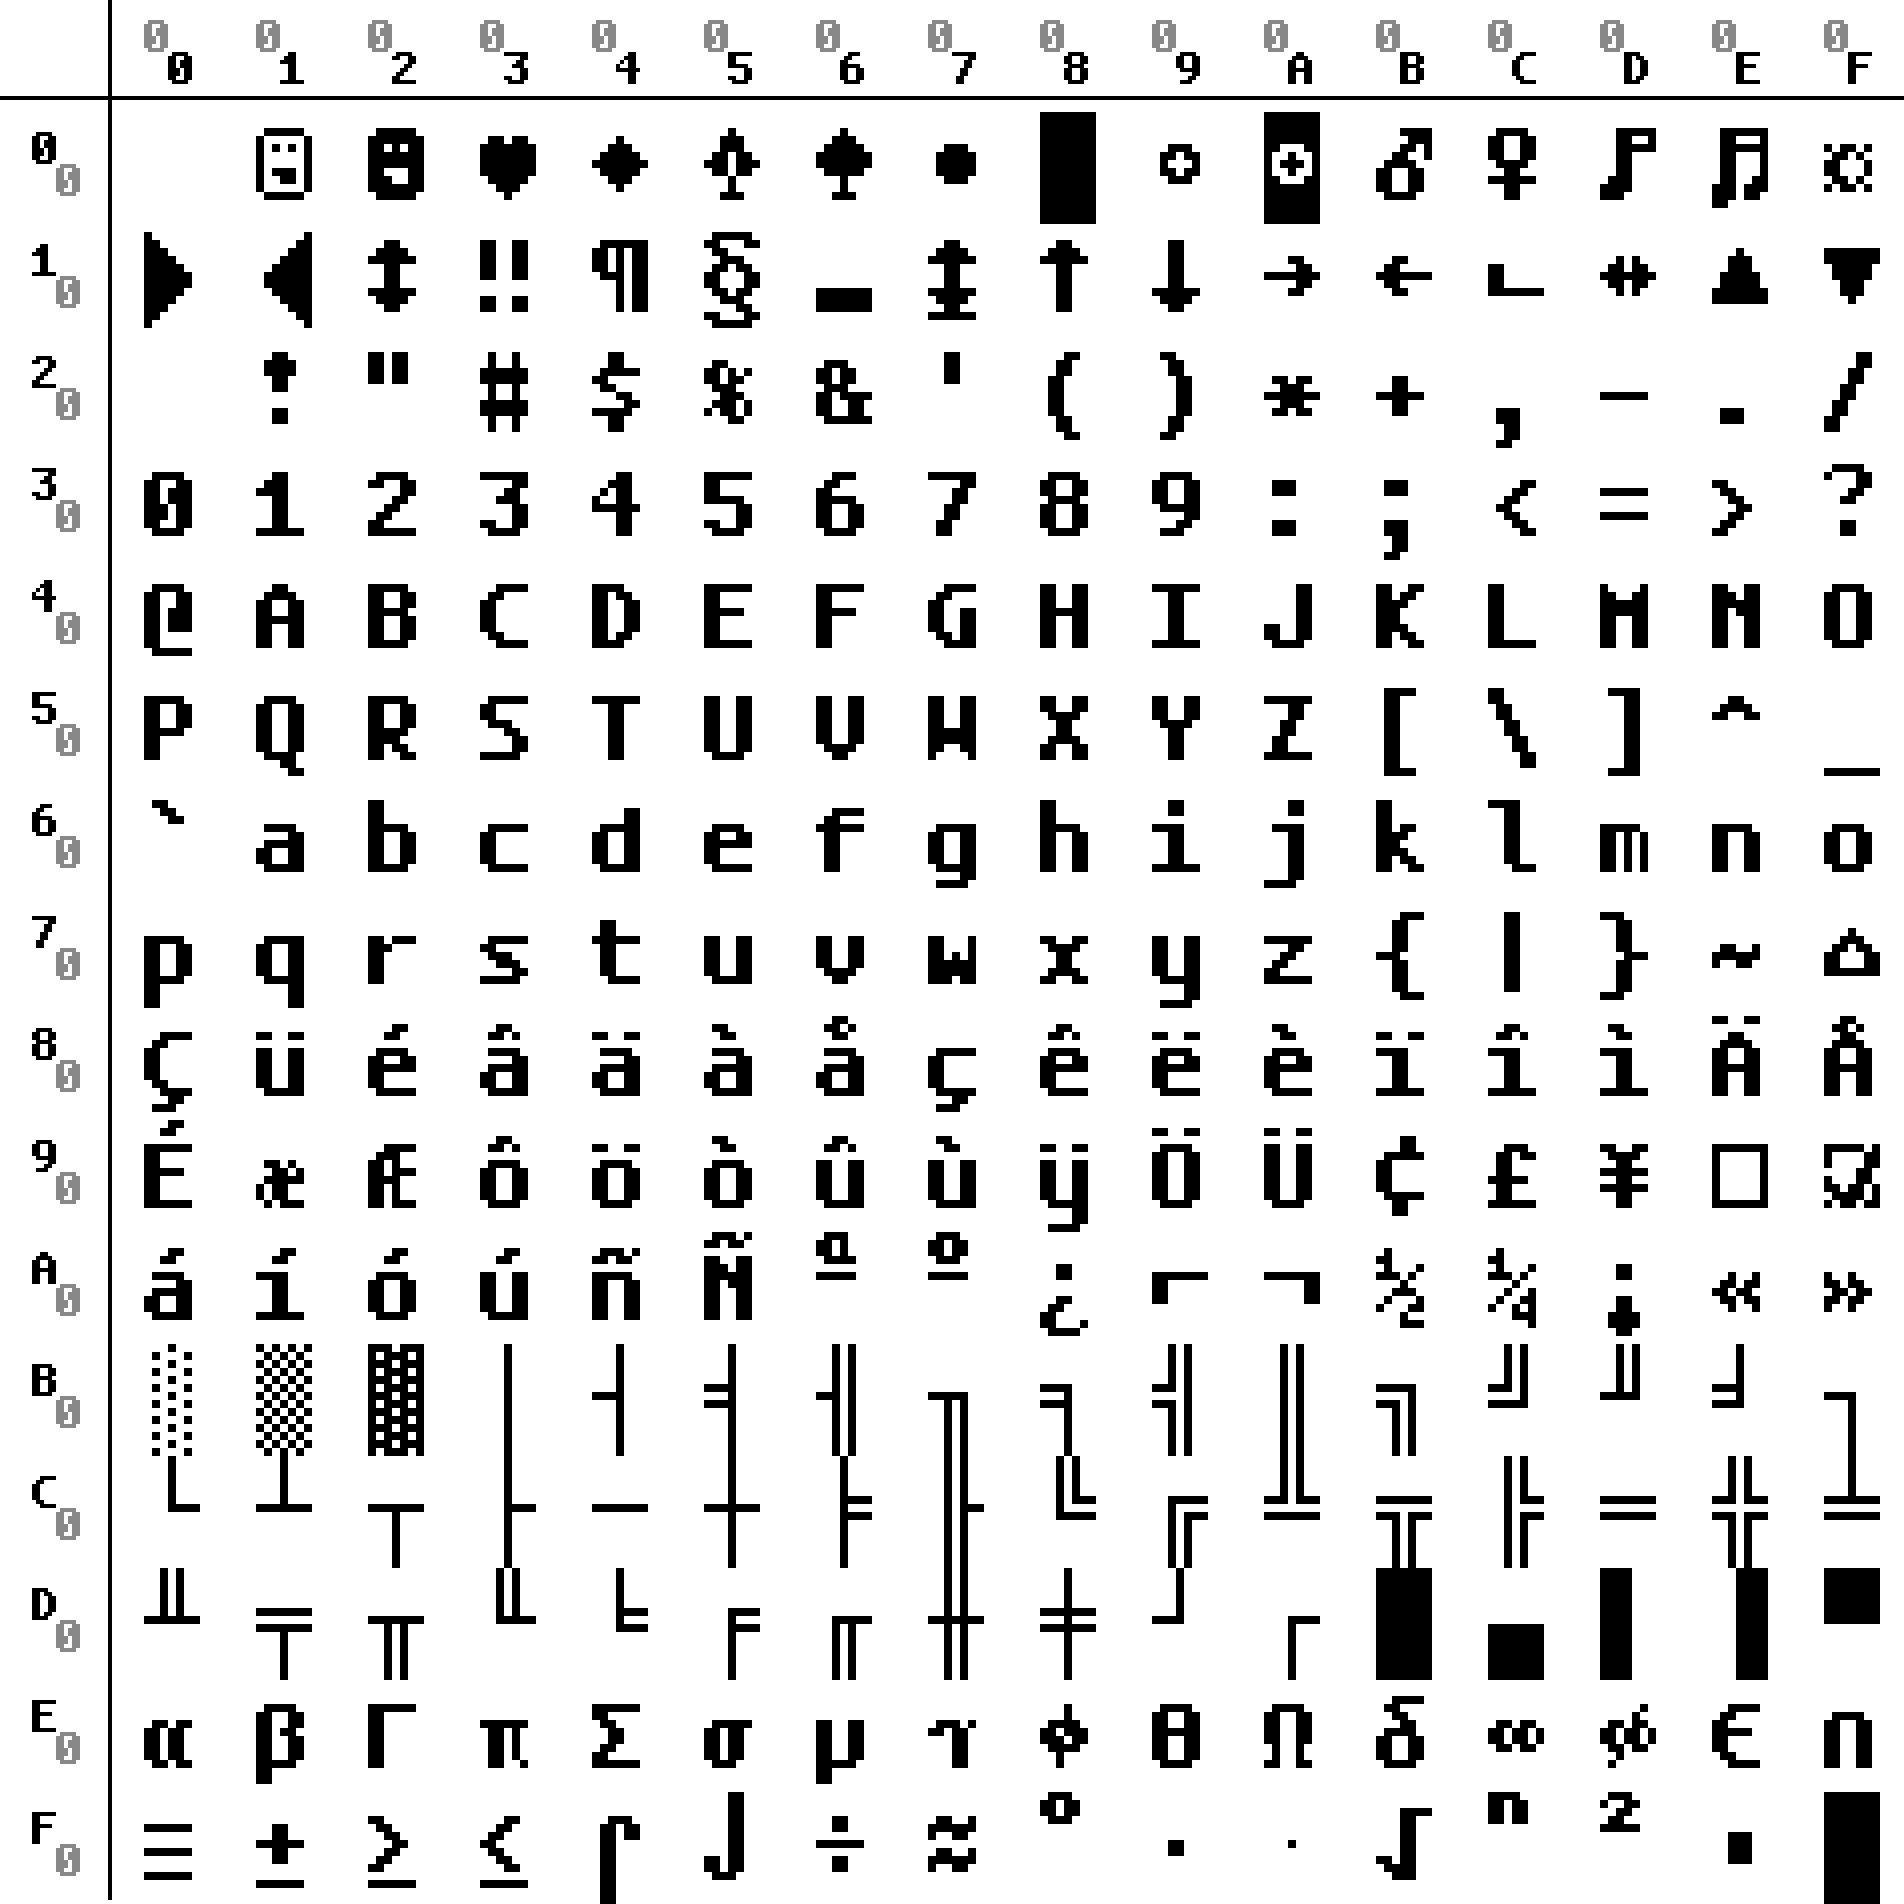
\includegraphics[width=\linewidth]{tsvmcp.png}
\captionof{figure}{\thismachine\ Character Map}
\label{fig:codepage}
}
\newpage

\section{Colour Palette}
\label{colourpalette}

\index{colour palette}By default the reference graphics adapter of the \thismachine\ uses following colour palette:

{\centering
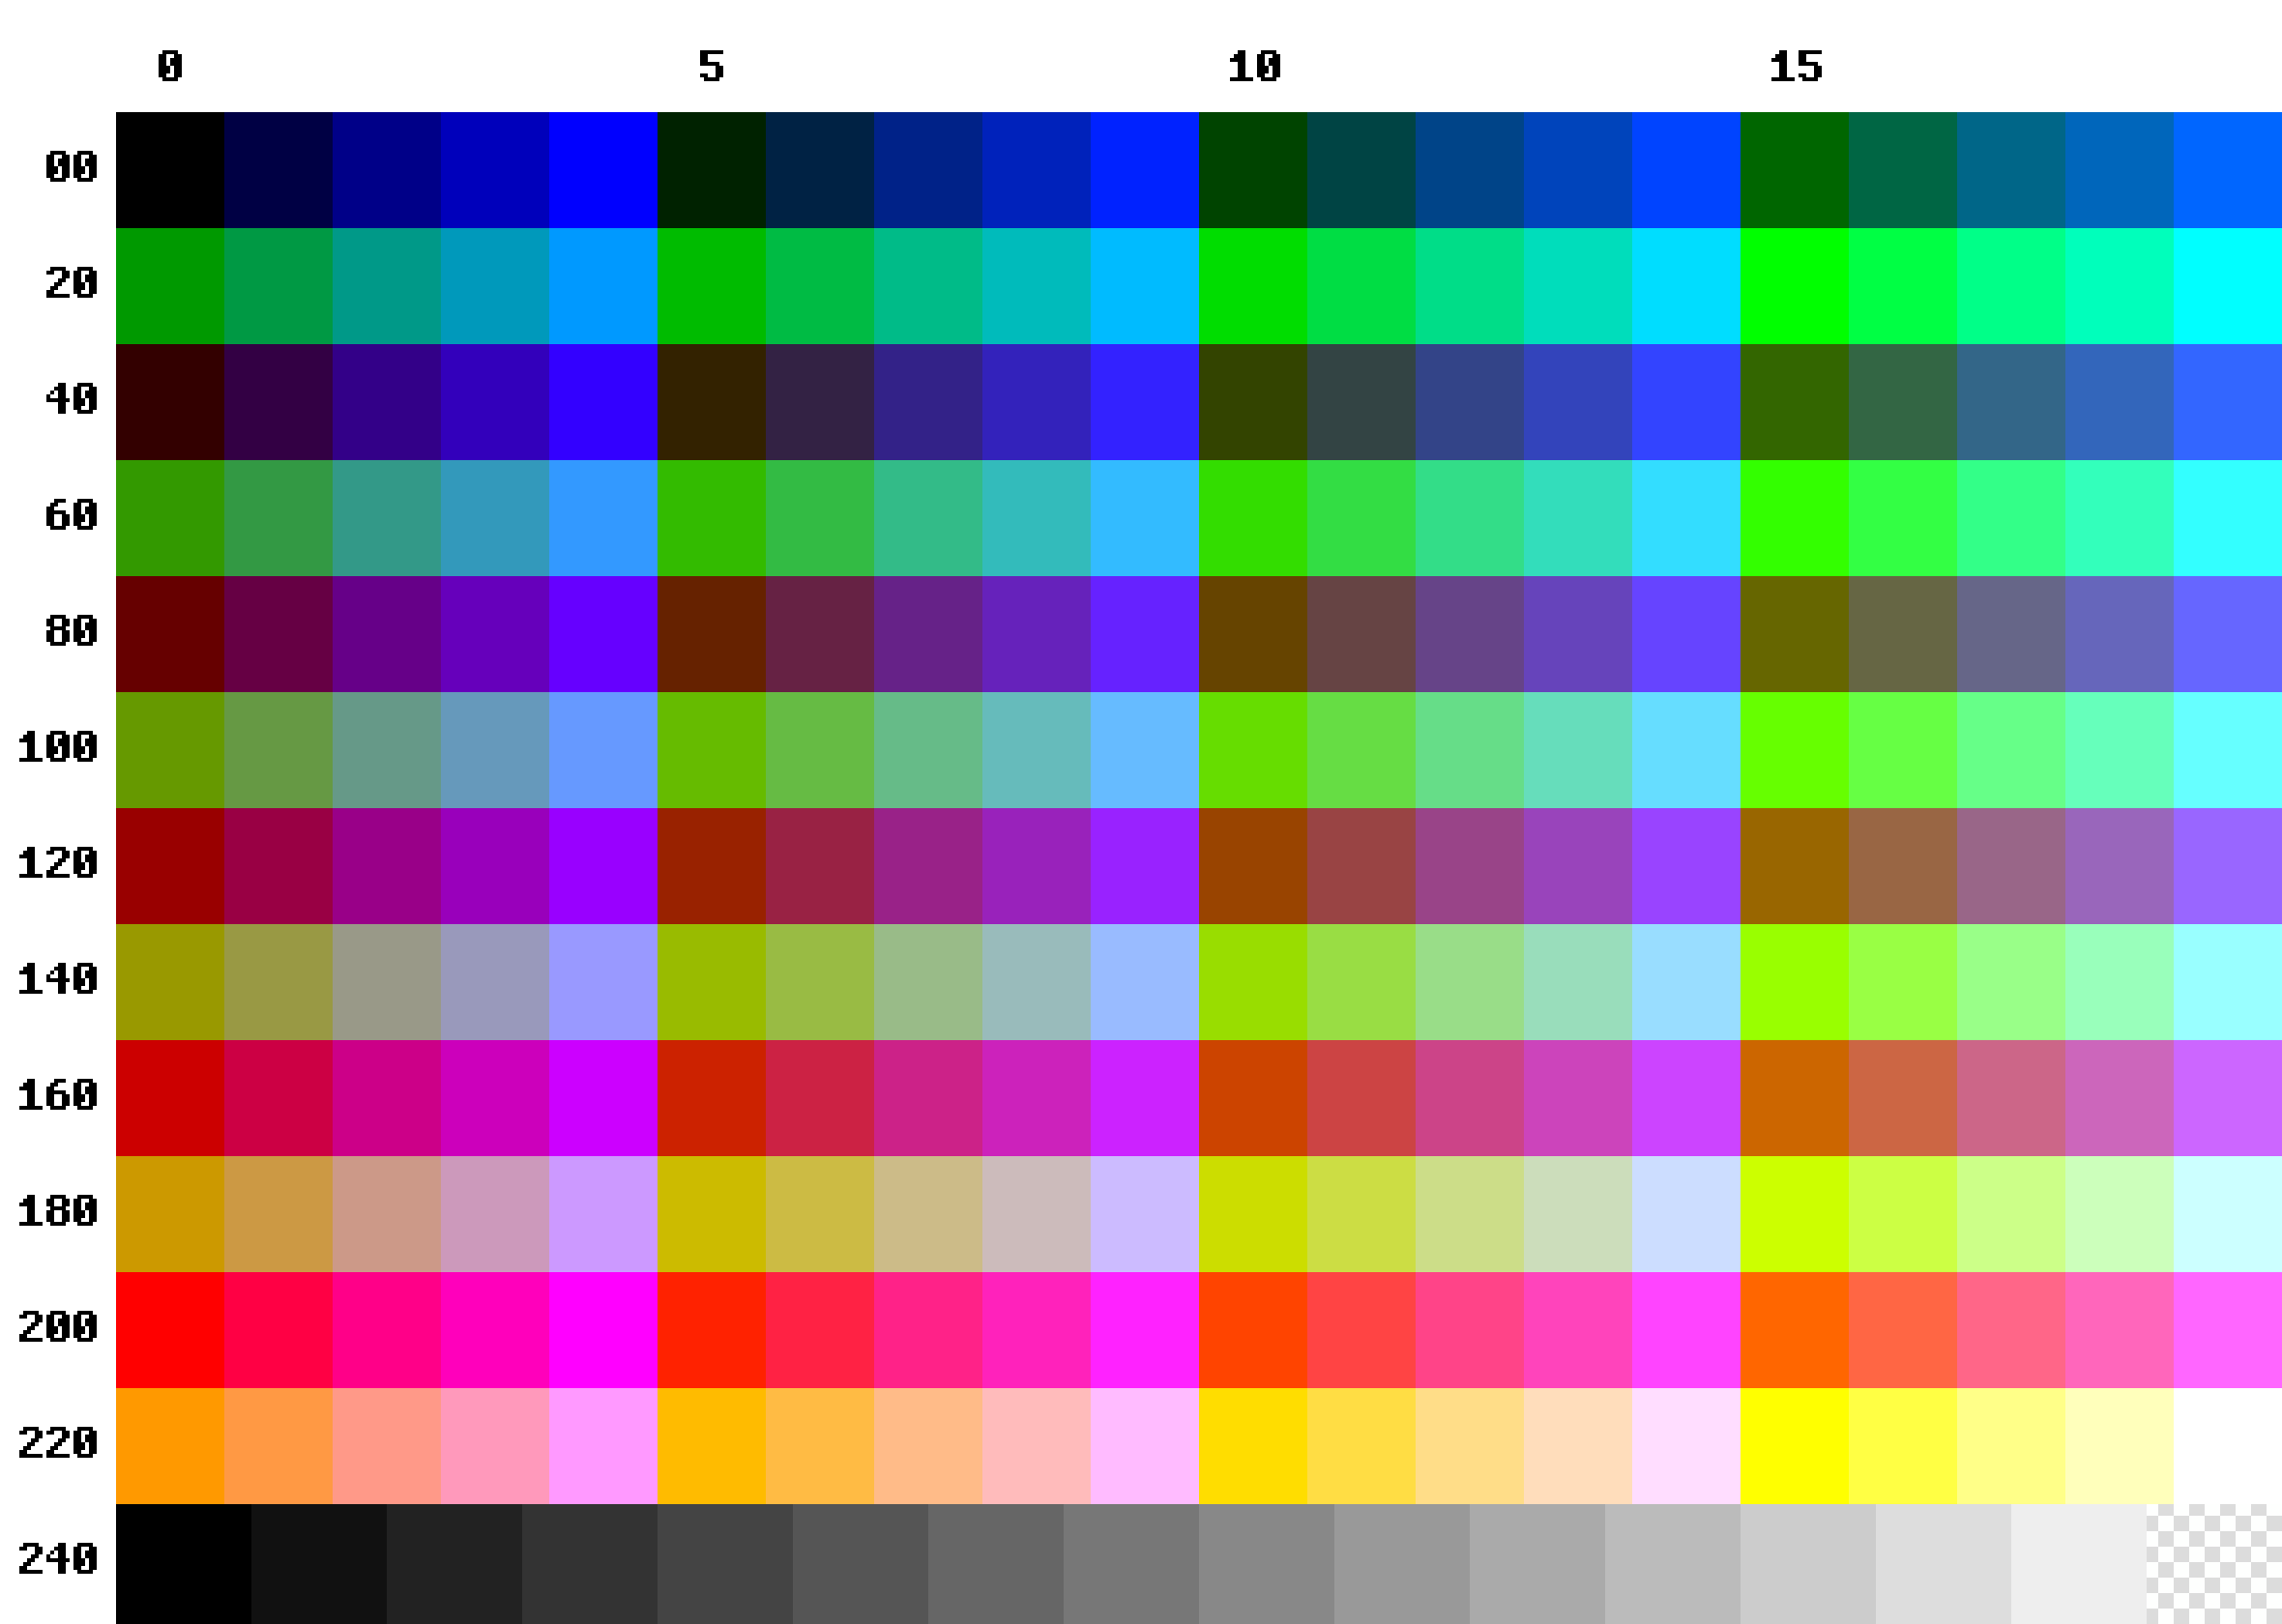
\includegraphics[width=\linewidth]{tsvmpal.png}
\captionof{figure}{\thismachine\ Colour Palette}
\label{fig:codepage}
}

{\centering
\fontsize{7pt}{0pt} % second argument is baselineskip but it's useless in table
\newlength{\extrarowheighttwo}
\setlength{\extrarowheighttwo}{\extrarowheight}
\setlength{\extrarowheight}{-0.2ex}

\begin{longtable}{*{2}{m{\textwidth}}}\hline
\endfirsthead
\endhead

\endfoot
\hline
\endlastfoot
\centering
\begin{tabulary}{\textwidth}{rl}
{\ttfamily 0} & {\ttfamily \#0000} \\
{\ttfamily 1} & {\ttfamily \#0004} \\
{\ttfamily 2} & {\ttfamily \#0008} \\
{\ttfamily 3} & {\ttfamily \#000B} \\
{\ttfamily 4} & {\ttfamily \#000F} \\
{\ttfamily 5} & {\ttfamily \#0020} \\
{\ttfamily 6} & {\ttfamily \#0024} \\
{\ttfamily 7} & {\ttfamily \#0028} \\
{\ttfamily 8} & {\ttfamily \#002B} \\
{\ttfamily 9} & {\ttfamily \#002F} \\
{\ttfamily 10} & {\ttfamily \#0040} \\
{\ttfamily 11} & {\ttfamily \#0044} \\
{\ttfamily 12} & {\ttfamily \#0048} \\
{\ttfamily 13} & {\ttfamily \#004B} \\
{\ttfamily 14} & {\ttfamily \#004F} \\
{\ttfamily 15} & {\ttfamily \#0060} \\
{\ttfamily 16} & {\ttfamily \#0064} \\
{\ttfamily 17} & {\ttfamily \#0068} \\
{\ttfamily 18} & {\ttfamily \#006B} \\
{\ttfamily 19} & {\ttfamily \#006F} \\
{\ttfamily 20} & {\ttfamily \#0090} \\
{\ttfamily 21} & {\ttfamily \#0094} \\
{\ttfamily 22} & {\ttfamily \#0098} \\
{\ttfamily 23} & {\ttfamily \#009B} \\
{\ttfamily 24} & {\ttfamily \#009F} \\
{\ttfamily 25} & {\ttfamily \#00B0} \\
{\ttfamily 26} & {\ttfamily \#00B4} \\
{\ttfamily 27} & {\ttfamily \#00B8} \\
{\ttfamily 28} & {\ttfamily \#00BB} \\
{\ttfamily 29} & {\ttfamily \#00BF} \\
{\ttfamily 30} & {\ttfamily \#00D0} \\
{\ttfamily 31} & {\ttfamily \#00D4} \\
{\ttfamily 32} & {\ttfamily \#00D8} \\
{\ttfamily 33} & {\ttfamily \#00DB} \\
{\ttfamily 34} & {\ttfamily \#00DF} \\
{\ttfamily 35} & {\ttfamily \#00F0} \\
{\ttfamily 36} & {\ttfamily \#00F4} \\
{\ttfamily 37} & {\ttfamily \#00F8} \\
{\ttfamily 38} & {\ttfamily \#00FB} \\
{\ttfamily 39} & {\ttfamily \#00FF} \\
{\ttfamily 40} & {\ttfamily \#0300} \\
{\ttfamily 41} & {\ttfamily \#0304} \\
{\ttfamily 42} & {\ttfamily \#0308} \\
\end{tabulary}
\begin{tabulary}{\textwidth}{|rl}
{\ttfamily 43} & {\ttfamily \#030B} \\
{\ttfamily 44} & {\ttfamily \#030F} \\
{\ttfamily 45} & {\ttfamily \#0320} \\
{\ttfamily 46} & {\ttfamily \#0324} \\
{\ttfamily 47} & {\ttfamily \#0328} \\
{\ttfamily 48} & {\ttfamily \#032B} \\
{\ttfamily 49} & {\ttfamily \#032F} \\
{\ttfamily 50} & {\ttfamily \#0340} \\
{\ttfamily 51} & {\ttfamily \#0344} \\
{\ttfamily 52} & {\ttfamily \#0348} \\
{\ttfamily 53} & {\ttfamily \#034B} \\
{\ttfamily 54} & {\ttfamily \#034F} \\
{\ttfamily 55} & {\ttfamily \#0360} \\
{\ttfamily 56} & {\ttfamily \#0364} \\
{\ttfamily 57} & {\ttfamily \#0368} \\
{\ttfamily 58} & {\ttfamily \#036B} \\
{\ttfamily 59} & {\ttfamily \#036F} \\
{\ttfamily 60} & {\ttfamily \#0390} \\
{\ttfamily 61} & {\ttfamily \#0394} \\
{\ttfamily 62} & {\ttfamily \#0398} \\
{\ttfamily 63} & {\ttfamily \#039B} \\
{\ttfamily 64} & {\ttfamily \#039F} \\
{\ttfamily 65} & {\ttfamily \#03B0} \\
{\ttfamily 66} & {\ttfamily \#03B4} \\
{\ttfamily 67} & {\ttfamily \#03B8} \\
{\ttfamily 68} & {\ttfamily \#03BB} \\
{\ttfamily 69} & {\ttfamily \#03BF} \\
{\ttfamily 70} & {\ttfamily \#03D0} \\
{\ttfamily 71} & {\ttfamily \#03D4} \\
{\ttfamily 72} & {\ttfamily \#03D8} \\
{\ttfamily 73} & {\ttfamily \#03DB} \\
{\ttfamily 74} & {\ttfamily \#03DF} \\
{\ttfamily 75} & {\ttfamily \#03F0} \\
{\ttfamily 76} & {\ttfamily \#03F4} \\
{\ttfamily 77} & {\ttfamily \#03F8} \\
{\ttfamily 78} & {\ttfamily \#03FB} \\
{\ttfamily 79} & {\ttfamily \#03FF} \\
{\ttfamily 80} & {\ttfamily \#0600} \\
{\ttfamily 81} & {\ttfamily \#0604} \\
{\ttfamily 82} & {\ttfamily \#0608} \\
{\ttfamily 83} & {\ttfamily \#060B} \\
{\ttfamily 84} & {\ttfamily \#060F} \\
{\ttfamily 85} & {\ttfamily \#0620} \\
\end{tabulary}
\begin{tabulary}{\textwidth}{|rl}
{\ttfamily 86} & {\ttfamily \#0624} \\
{\ttfamily 87} & {\ttfamily \#0628} \\
{\ttfamily 88} & {\ttfamily \#062B} \\
{\ttfamily 89} & {\ttfamily \#062F} \\
{\ttfamily 90} & {\ttfamily \#0640} \\
{\ttfamily 91} & {\ttfamily \#0644} \\
{\ttfamily 92} & {\ttfamily \#0648} \\
{\ttfamily 93} & {\ttfamily \#064B} \\
{\ttfamily 94} & {\ttfamily \#064F} \\
{\ttfamily 95} & {\ttfamily \#0660} \\
{\ttfamily 96} & {\ttfamily \#0664} \\
{\ttfamily 97} & {\ttfamily \#0668} \\
{\ttfamily 98} & {\ttfamily \#066B} \\
{\ttfamily 99} & {\ttfamily \#066F} \\
{\ttfamily 100} & {\ttfamily \#0690} \\
{\ttfamily 101} & {\ttfamily \#0694} \\
{\ttfamily 102} & {\ttfamily \#0698} \\
{\ttfamily 103} & {\ttfamily \#069B} \\
{\ttfamily 104} & {\ttfamily \#069F} \\
{\ttfamily 105} & {\ttfamily \#06B0} \\
{\ttfamily 106} & {\ttfamily \#06B4} \\
{\ttfamily 107} & {\ttfamily \#06B8} \\
{\ttfamily 108} & {\ttfamily \#06BB} \\
{\ttfamily 109} & {\ttfamily \#06BF} \\
{\ttfamily 110} & {\ttfamily \#06D0} \\
{\ttfamily 111} & {\ttfamily \#06D4} \\
{\ttfamily 112} & {\ttfamily \#06D8} \\
{\ttfamily 113} & {\ttfamily \#06DB} \\
{\ttfamily 114} & {\ttfamily \#06DF} \\
{\ttfamily 115} & {\ttfamily \#06F0} \\
{\ttfamily 116} & {\ttfamily \#06F4} \\
{\ttfamily 117} & {\ttfamily \#06F8} \\
{\ttfamily 118} & {\ttfamily \#06FB} \\
{\ttfamily 119} & {\ttfamily \#06FF} \\
{\ttfamily 120} & {\ttfamily \#0900} \\
{\ttfamily 121} & {\ttfamily \#0904} \\
{\ttfamily 122} & {\ttfamily \#0908} \\
{\ttfamily 123} & {\ttfamily \#090B} \\
{\ttfamily 124} & {\ttfamily \#090F} \\
{\ttfamily 125} & {\ttfamily \#0920} \\
{\ttfamily 126} & {\ttfamily \#0924} \\
{\ttfamily 127} & {\ttfamily \#0928} \\
{\ttfamily 128} & {\ttfamily \#092B} \\
\end{tabulary}
\begin{tabulary}{\textwidth}{|rl}
{\ttfamily 129} & {\ttfamily \#092F} \\
{\ttfamily 130} & {\ttfamily \#0940} \\
{\ttfamily 131} & {\ttfamily \#0944} \\
{\ttfamily 132} & {\ttfamily \#0948} \\
{\ttfamily 133} & {\ttfamily \#094B} \\
{\ttfamily 134} & {\ttfamily \#094F} \\
{\ttfamily 135} & {\ttfamily \#0960} \\
{\ttfamily 136} & {\ttfamily \#0964} \\
{\ttfamily 137} & {\ttfamily \#0968} \\
{\ttfamily 138} & {\ttfamily \#096B} \\
{\ttfamily 139} & {\ttfamily \#096F} \\
{\ttfamily 140} & {\ttfamily \#0990} \\
{\ttfamily 141} & {\ttfamily \#0994} \\
{\ttfamily 142} & {\ttfamily \#0998} \\
{\ttfamily 143} & {\ttfamily \#099B} \\
{\ttfamily 144} & {\ttfamily \#099F} \\
{\ttfamily 145} & {\ttfamily \#09B0} \\
{\ttfamily 146} & {\ttfamily \#09B4} \\
{\ttfamily 147} & {\ttfamily \#09B8} \\
{\ttfamily 148} & {\ttfamily \#09BB} \\
{\ttfamily 149} & {\ttfamily \#09BF} \\
{\ttfamily 150} & {\ttfamily \#09D0} \\
{\ttfamily 151} & {\ttfamily \#09D4} \\
{\ttfamily 152} & {\ttfamily \#09D8} \\
{\ttfamily 153} & {\ttfamily \#09DB} \\
{\ttfamily 154} & {\ttfamily \#09DF} \\
{\ttfamily 155} & {\ttfamily \#09F0} \\
{\ttfamily 156} & {\ttfamily \#09F4} \\
{\ttfamily 157} & {\ttfamily \#09F8} \\
{\ttfamily 158} & {\ttfamily \#09FB} \\
{\ttfamily 159} & {\ttfamily \#09FF} \\
{\ttfamily 160} & {\ttfamily \#0C00} \\
{\ttfamily 161} & {\ttfamily \#0C04} \\
{\ttfamily 162} & {\ttfamily \#0C08} \\
{\ttfamily 163} & {\ttfamily \#0C0B} \\
{\ttfamily 164} & {\ttfamily \#0C0F} \\
{\ttfamily 165} & {\ttfamily \#0C20} \\
{\ttfamily 166} & {\ttfamily \#0C24} \\
{\ttfamily 167} & {\ttfamily \#0C28} \\
{\ttfamily 168} & {\ttfamily \#0C2B} \\
{\ttfamily 169} & {\ttfamily \#0C2F} \\
{\ttfamily 170} & {\ttfamily \#0C40} \\
{\ttfamily 171} & {\ttfamily \#0C44} \\
\end{tabulary}
\begin{tabulary}{\textwidth}{|rl}
{\ttfamily 172} & {\ttfamily \#0C48} \\
{\ttfamily 173} & {\ttfamily \#0C4B} \\
{\ttfamily 174} & {\ttfamily \#0C4F} \\
{\ttfamily 175} & {\ttfamily \#0C60} \\
{\ttfamily 176} & {\ttfamily \#0C64} \\
{\ttfamily 177} & {\ttfamily \#0C68} \\
{\ttfamily 178} & {\ttfamily \#0C6B} \\
{\ttfamily 179} & {\ttfamily \#0C6F} \\
{\ttfamily 180} & {\ttfamily \#0C90} \\
{\ttfamily 181} & {\ttfamily \#0C94} \\
{\ttfamily 182} & {\ttfamily \#0C98} \\
{\ttfamily 183} & {\ttfamily \#0C9B} \\
{\ttfamily 184} & {\ttfamily \#0C9F} \\
{\ttfamily 185} & {\ttfamily \#0CB0} \\
{\ttfamily 186} & {\ttfamily \#0CB4} \\
{\ttfamily 187} & {\ttfamily \#0CB8} \\
{\ttfamily 188} & {\ttfamily \#0CBB} \\
{\ttfamily 189} & {\ttfamily \#0CBF} \\
{\ttfamily 190} & {\ttfamily \#0CD0} \\
{\ttfamily 191} & {\ttfamily \#0CD4} \\
{\ttfamily 192} & {\ttfamily \#0CD8} \\
{\ttfamily 193} & {\ttfamily \#0CDB} \\
{\ttfamily 194} & {\ttfamily \#0CDF} \\
{\ttfamily 195} & {\ttfamily \#0CF0} \\
{\ttfamily 196} & {\ttfamily \#0CF4} \\
{\ttfamily 197} & {\ttfamily \#0CF8} \\
{\ttfamily 198} & {\ttfamily \#0CFB} \\
{\ttfamily 199} & {\ttfamily \#0CFF} \\
{\ttfamily 200} & {\ttfamily \#0F00} \\
{\ttfamily 201} & {\ttfamily \#0F04} \\
{\ttfamily 202} & {\ttfamily \#0F08} \\
{\ttfamily 203} & {\ttfamily \#0F0B} \\
{\ttfamily 204} & {\ttfamily \#0F0F} \\
{\ttfamily 205} & {\ttfamily \#0F20} \\
{\ttfamily 206} & {\ttfamily \#0F24} \\
{\ttfamily 207} & {\ttfamily \#0F28} \\
{\ttfamily 208} & {\ttfamily \#0F2B} \\
{\ttfamily 209} & {\ttfamily \#0F2F} \\
{\ttfamily 210} & {\ttfamily \#0F40} \\
{\ttfamily 211} & {\ttfamily \#0F44} \\
{\ttfamily 212} & {\ttfamily \#0F48} \\
{\ttfamily 213} & {\ttfamily \#0F4B} \\
{\ttfamily 214} & {\ttfamily \#0F4F} \\
\end{tabulary}
\begin{tabulary}{\textwidth}{|rl}
{\ttfamily 215} & {\ttfamily \#0F60} \\
{\ttfamily 216} & {\ttfamily \#0F64} \\
{\ttfamily 217} & {\ttfamily \#0F68} \\
{\ttfamily 218} & {\ttfamily \#0F6B} \\
{\ttfamily 219} & {\ttfamily \#0F6F} \\
{\ttfamily 220} & {\ttfamily \#0F90} \\
{\ttfamily 221} & {\ttfamily \#0F94} \\
{\ttfamily 222} & {\ttfamily \#0F98} \\
{\ttfamily 223} & {\ttfamily \#0F9B} \\
{\ttfamily 224} & {\ttfamily \#0F9F} \\
{\ttfamily 225} & {\ttfamily \#0FB0} \\
{\ttfamily 226} & {\ttfamily \#0FB4} \\
{\ttfamily 227} & {\ttfamily \#0FB8} \\
{\ttfamily 228} & {\ttfamily \#0FBB} \\
{\ttfamily 229} & {\ttfamily \#0FBF} \\
{\ttfamily 230} & {\ttfamily \#0FD0} \\
{\ttfamily 231} & {\ttfamily \#0FD4} \\
{\ttfamily 232} & {\ttfamily \#0FD8} \\
{\ttfamily 233} & {\ttfamily \#0FDB} \\
{\ttfamily 234} & {\ttfamily \#0FDF} \\
{\ttfamily 235} & {\ttfamily \#0FF0} \\
{\ttfamily 236} & {\ttfamily \#0FF4} \\
{\ttfamily 237} & {\ttfamily \#0FF8} \\
{\ttfamily 238} & {\ttfamily \#0FFB} \\
{\ttfamily 239} & {\ttfamily \#0FFF} \\
{\ttfamily 240} & {\ttfamily \#0000} \\
{\ttfamily 241} & {\ttfamily \#0111} \\
{\ttfamily 242} & {\ttfamily \#0222} \\
{\ttfamily 243} & {\ttfamily \#0333} \\
{\ttfamily 244} & {\ttfamily \#0444} \\
{\ttfamily 245} & {\ttfamily \#0555} \\
{\ttfamily 246} & {\ttfamily \#0666} \\
{\ttfamily 247} & {\ttfamily \#0777} \\
{\ttfamily 248} & {\ttfamily \#0888} \\
{\ttfamily 249} & {\ttfamily \#0999} \\
{\ttfamily 250} & {\ttfamily \#0AAA} \\
{\ttfamily 251} & {\ttfamily \#0BBB} \\
{\ttfamily 252} & {\ttfamily \#0CCC} \\
{\ttfamily 253} & {\ttfamily \#0DDD} \\
{\ttfamily 254} & {\ttfamily \#0EEE} \\
{\ttfamily 255} & {\ttfamily \#1000} \\
\, & \, \\
\, & \, \\
\end{tabulary}
\end{longtable}

\captionof{table}{Index--ARGB Table of the Colour Palette}
}

\setlength{\extrarowheight}{\extrarowheighttwo}


\part{More Goodies}

\chapter{99 Bottles of Beer}
This is a sample program that prints out the infamous \emph{99 Bottles of Beer}.

\begin{lstlisting}
10 FOR I = 99 TO 1 STEP -1
20 MODE = 1
30 GOSUB 120
40 PRINT I;" bottle";BOTTLES;" of beer on the wall, ";i;" bottle";BOTTLES;" of beer."
50 MODE = 2
60 GOSUB 120
70 PRINT "Take one down and pass it around, ";(I-1);" bottle";BOTTLES;" of beer on the wall."
80 NEXT
90 PRINT "No more bottles of beer on the wall, no more bottles of beer."
100 PRINT "Go to the store and buy some more. 99 bottles of beer on the wall."
110 END
120 IF I == MODE THEN BOTTLES = "" ELSE BOTTLES = "s"
130 RETURN
\end{lstlisting}


\chapter{Amazing}
This is a sample program that draw a randomised maze. The original program was on \emph{BASIC Computer Games: Microcomputer Edition} and was translated into \tbas.

\begin{lstlisting}
1 OPTIONBASE 1
10 PRINT SPC(28);"AMAZING PROGRAM"
20 PRINT SPC(15);"CREATIVE COMPUTING  MORRISTOWN, NEW JERSEY"
30 PRINT:PRINT:PRINT
100 PRINT "WHAT ARE YOUR WIDTH";:INPUT H
102 PRINT "WHAT ARE YOUR LENGTH";:INPUT V
105 IF H<>1 AND V<>1 THEN GOTO 110
106 PRINT "MEANINGLESS DIMENSIONS.  TRY AGAIN.":GOTO 100
110 WS=DIM(H,V):VS=DIM(H,V)
120 PRINT:PRINT:PRINT:PRINT
160 Q=0:Z=0:X=INT(RND(1)*H+1)
165 FOR I=1 TO H
170   IF I==X THEN GOTO 173
171   PRINT ".--";
172   GOTO 175
173   PRINT ".  ";
180 NEXT
190 PRINT "."
195 C=1:WS(X,1)=C:C=C+1
200 R=X:S=1:GOTO 260
210 IF R<>H THEN GOTO 240
215 IF S<>V THEN GOTO 230
220 R=1:S=1
222 GOTO 250
230 R=1:S=S+1:GOTO 250
240 R=R+1
250 IF WS(R,S)==0 THEN GOTO 210
260 IF R-1==0 THEN GOTO 530
265 IF WS(R-1,S)<>0 THEN GOTO 530
270 IF S-1==0 THEN GOTO 390
280 IF WS(R,S-1)<>0 THEN GOTO 390
290 IF R==H THEN GOTO 330
300 IF WS(R+1,S)<>0 THEN GOTO 330
310 X=INT(RND(1)*3+1)
320 ON X GOTO 790,820,860
334 IF Z==1 THEN GOTO 370
338 Q=1:GOTO 350
340 IF WS(R,S+1)<>0 THEN GOTO 370
350 X=INT(RND(1)*3+1)
360 ON X GOTO 790,820,910
370 X=INT(RND(1)*2+1)
380 ON X GOTO 790,820
390 IF R==H THEN GOTO 470
400 IF WS(R+1,S)<>0 THEN GOTO 470
405 IF S<>V THEN GOTO 420
410 IF Z==1 THEN GOTO 450
415 Q=1:GOTO 430
420 IF WS(R,S+1)<>0 THEN GOTO 450
430 X=INT(RND(1)*3+1)
440 ON X GOTO 790,860,910
450 X=INT(RND(1)*2+1)
460 ON X GOTO 790,860
470 IF S<>V THEN GOTO 490
480 IF Z==1 THEN GOTO 520
485 Q=1:GOTO 500
490 IF WS(R,S+1)<>0 THEN GOTO 520
500 X=INT(RND(1)*2+1)
510 ON X GOTO 790,910
520 GOTO 790
530 IF S-1==0 THEN GOTO 670
540 IF WS(R,S-1)<>0 THEN GOTO 670
545 IF R==H THEN GOTO 610
547 IF WS(R+1,S)<>0 THEN GOTO 610
550 IF S<>V THEN GOTO 560
552 IF Z==1 THEN GOTO 590
554 Q=1:GOTO 570
560 IF WS(R,S+1)<>0 THEN GOTO 590
570 X=INT(RND(1)*3+1)
580 ON X GOTO 820,860,910
590 X=INT(RND(1)*2+1)
600 ON X GOTO 820,860
610 IF S<>V THEN GOTO 630
620 IF Z==1 THEN GOTO 660
625 Q=1:GOTO 640
630 IF WS(R,S+1)<>0 THEN GOTO 660
640 X=INT(RND(1)*2+1)
650 ON X GOTO 820,910
660 GOTO 820
670 IF R==H THEN GOTO 740
680 IF WS(R+1,S)<>0 THEN GOTO 740
685 IF S<>V THEN GOTO 700
690 IF Z==1 THEN GOTO 730
695 Q=1:GOTO 830
700 IF WS(R,S+1)<>0 THEN GOTO 730
710 X=INT(RND(1)*2+1)
720 ON X GOTO 860,910
730 GOTO 860
740 IF S<>V THEN GOTO 760
750 IF Z==1 THEN GOTO 780
755 Q=1:GOTO 770
760 IF WS(R,S+1)<>0 THEN GOTO 780
770 GOTO 910
780 GOTO 1000
790 WS(R-1,S)=C
800 C=C+1:VS(R-1,S)=2:R=R-1
810 IF C==H*V+1 THEN GOTO 1010
815 Q=0:GOTO 260
820 WS(R,S-1)=C
830 C=C+1
840 VS(R,S-1)=1:S=S-1:IF C==H*V+1 THEN GOTO 1010
850 Q=0:GOTO 260
860 WS(R+1,S)=C
870 C=C+1:IF VS(R,S)==0 THEN GOTO 880
875 VS(R,S)=3:GOTO 890
880 VS(R,S)=2
890 R=R+1
900 IF C==H*V+1 THEN GOTO 1010
905 GOTO 530
910 IF Q==1 THEN GOTO 960
920 WS(R,S+1)=C:C=C+1:IF VS(R,S)==0 THEN GOTO 940
930 VS(R,S)=3:GOTO 950
940 VS(R,S)=1
950 S=S+1:IF C==H*V+1 THEN GOTO 1010
955 GOTO 260
960 Z=1
970 IF VS(R,S)==0 THEN GOTO 980
975 VS(R,S)=3:Q=0:GOTO 1000
980 VS(R,S)=1:Q=0:R=1:S=1:GOTO 250
1000 GOTO 210
1010 FOR J=1 TO V
1011   PRINT "|";
1012   FOR I=1 TO H
1013     IF VS(I,J)<2 THEN GOTO 1030
1020     PRINT "   ";
1021     GOTO 1040
1030     PRINT "  |";
1040   NEXT
1041   PRINT
1043   FOR I=1 TO H
1045     IF VS(I,J)==0 THEN GOTO 1060
1050     IF VS(I,J)==2 THEN GOTO 1060
1051     PRINT ":  ";
1052     GOTO 1070
1060     PRINT ":--";
1070   NEXT
1071   PRINT "."
1072 NEXT
1073 END
\end{lstlisting}


\chapter{Hamurabi}
This is a sample program that is the \emph{Hamurabi} game. The original program was on \emph{BASIC Computer Games: Microcomputer Edition} and was translated into \tbas.

This game is considered as the grand ancestor of the strategy, simulation and city-building games; in fact it's so great it has got its own Wikipedia article.

\begin{lstlisting}
10 PRINT SPC(32);"HAMURABI"
20 PRINT SPC(15);"CREATIVE COMPUTING  MORRISTOWN, NEW JERSEY"
30 PRINT:PRINT:PRINT
80 PRINT "TRY YOUR HAND AT GOVERNING ANCIENT SUMERIA"
90 PRINT "FOR A TEN-YEAR TERM OF OFFICE.":PRINT
95 D1=0:P1=0
100 Z=0:P=95:S=2800:H=3000:E=H-S
110 Y=3:A=H/Y:I=5:Q=1
210 D=0
215 PRINT:PRINT:PRINT "HAMURABI:  I BEG TO REPORT TO YOU,":Z=Z+1
217 PRINT "IN YEAR ";Z;", ";D;" PEOPLE STARVED, ";I;" CAME TO THE CITY,"
220 P=P+I
227 IF Q>0 THEN GOTO 230
228 P=INT(P/2)
229 PRINT "A HORRIBLE PLAGUE STRUCK!  HALF THE PEOPLE DIED."
230 PRINT "POPULATION IS NOW ";P
232 PRINT "THE CITY NOW OWNS ";A;" ACRES."
235 PRINT "YOU HARVESTED ";Y;" BUSHELS PER ACRE."
250 PRINT "THE RATS ATE ";E;" BUSHELS."
260 PRINT "YOU NOW HAVE ";S;" BUSHELS IN STORE."
261 PRINT
270 IF Z==11 THEN GOTO 860
310 C=INT(10*RND(1))
311 Y=C+17
312 PRINT "LAND IS TRADING AT ";Y;" BUSHELS PER ACRE."
320 PRINT "HOW MANY ACRES DO YOU WISH TO BUY";
321 INPUT Q
322 IF Q<0 THEN GOTO 850
323 IF Y*Q<=S THEN GOTO 330
324 GOSUB 710
325 GOTO 320
330 IF Q==0 THEN GOTO 340
331 A=A+Q:S=S-Y*Q:C=0
334 GOTO 400
340 PRINT "HOW MANY ACRES DO YOU WISH TO SELL";
341 INPUT Q
342 IF Q<0 THEN GOTO 850
343 IF Q<A THEN GOTO 350
344 GOSUB 720
345 GOTO 340
350 A=A-Q:S=S+Y*Q:C=0
400 PRINT
410 PRINT "HOW MANY BUSHELS DO YOU WISH TO FEED YOUR PEOPLE";
411 INPUT Q
412 IF Q<0 THEN GOTO 850
418 REM *** TRYING TO USE MORE GRAIN THAN IS IN SILOS?
420 IF Q<=S THEN GOTO 430
421 GOSUB 710
422 GOTO 410
430 S=S-Q:C=1:PRINT
440 PRINT "HOW MANY ACRES DO YOU WISH TO PLANT WITH SEED";
441 INPUT D
442 IF D==0 THEN GOTO 511
443 IF D<0 THEN GOTO 850
444 REM *** TRYING TO PLANT MORE ACRES THAN YOU OWN?
445 IF D<=A THEN GOTO 450
446 GOSUB 720
447 GOTO 440
449 REM *** ENOUGH GRAIN FOR SEED?
450 IF INT(D/2)<=S THEN GOTO 455
452 GOSUB 710
453 GOTO 440
454 REM *** ENOUGH PEOPLE TO TEND THE CROPS?
455 IF D<10*P THEN GOTO 510
460 PRINT "BUT YOU HAVE ONLY ";P;" PEOPLE TO TEND THE FIELDS!  NOW THEN,"
470 GOTO 440
510 S=S-INT(D/2)
511 GOSUB 800
512 REM *** A BOUNTIFUL HARVEST!
515 Y=C:H=D*Y:E=0
521 GOSUB 800
522 IF INT(C/2)<>C/2 THEN GOTO 530
523 REM *** RATS ARE RUNNING WILD!!
525 E=INT(S/C)
530 S=S-E+H
531 GOSUB 800
532 REM *** LET'S HAVE SOME BABIES
533 I=INT(C*(20*A+S)/P/100+1)
539 REM *** HOW MANY PEOPLE HAD FULL TUMMIES?
540 C=INT(Q/20)
541 REM *** HORROS, A 15% CHANCE OF PLAGUE
542 Q=INT(10*(2*RND(1)-0.3))
550 IF P<C THEN GOTO 210
551 REM *** STARVE ENOUGH FOR IMPEACHMENT?
552 D=P-C
553 IF D>0.45*P THEN GOTO 560
554 P1=((Z-1)*P1+D*100/P)/Z
555 P=C
556 D1=D1+D
557 GOTO 215
560 PRINT
561 PRINT "YOU STARVED ";D;" PEOPLE IN ONE YEAR!!!"
565 PRINT "DUE TO THIS EXTREME MISMANAGEMENT YOU HAVE NOT ONLY"
566 PRINT "BEEN IMPEACHED AND THROWN OUT OF OFFICE BUT YOU HAVE"
567 PRINT "ALSO BEEN DECLARED NATIONAL FINK!!!!"
568 GOTO 990
710 PRINT "HAMURABI:  THINK AGAIN.  YOU HAVE ONLY"
711 PRINT S;" BUSHELS OF GRAIN.  NOW THEN,"
712 RETURN
720 PRINT "HAMURABI:  THINK AGAIN.  YOU OWN ONLY ";A;" ACRES.  NOW THEN,"
730 RETURN
800 C=INT(RND(1)*5)+1
801 RETURN
850 PRINT
851 PRINT "HAMURABI:  I CANNOT DO WHAT YOU WISH."
855 PRINT "GET YOURSELF ANOTHER STEWARD!!!!!"
857 GOTO 990
860 PRINT "IN YOUR 10-YEAR TERM OF OFFICE, ";P1;" PERCENT OF THE"
862 PRINT "POPULATION STARVED PER YEAR ON THE AVERAGE, I.E. A TOTAL OF"
865 PRINT D1;"PEOPLE DIED!!"
866 L=A/P
870 PRINT "YOU STARTED WITH 10 ACRES PER PERSON AND ENDED WITH"
875 PRINT L;"ACRES PER PERSON."
876 PRINT
880 IF P1>33 THEN GOTO 565
885 IF L<7 THEN GOTO 565
890 IF P1>10 THEN GOTO 940
892 IF L<9 THEN GOTO 940
895 IF P1>3 THEN GOTO 960
896 IF L<10 THEN GOTO 960
900 PRINT "A FANTASTIC PERFORMANCE!!!  CHARLEMANGE, DISRAELI, AND"
905 PRINT "JEFFERSON COMBINED COULD NOT HAVE DONE BETTER!"
906 GOTO 990
940 PRINT "YOUR HEAVY-HANDED PERFORMANCE SMACKS OF NERO AND IVAN IV."
945 PRINT "THE PEOPLE (REMIANING) FIND YOU AN UNPLEASANT RULER, AND,"
950 PRINT "FRANKLY, HATE YOUR GUTS!!"
951 GOTO 990
960 PRINT "YOUR PERFORMANCE COULD HAVE BEEN SOMEWHAT BETTER, BUT"
965 PRINT "REALLY WASN'T TOO BAD AT ALL. ";INT(P*0.8*RND(1));" PEOPLE"
970 PRINT "WOULD DEARLY LIKE TO SEE YOU ASSASSINATED BUT WE ALL HAVE OUR"
975 PRINT "TRIVIAL PROBLEMS."
990 PRINT
991 FOR N=1 TO 10
992 PRINT EMIT(7;)
993 NEXT
995 PRINT "SO LONG FOR NOW."
996 PRINT
999 END
\end{lstlisting}


\chapter{Hangman}
This is a sample program that is the \emph{Hangman} game. The original program was on \emph{BASIC Computer Games: Microcomputer Edition} and was translated into \tbas.

\begin{lstlisting}
1 OPTIONBASE 1
10 PRINT SPC(32);"HANGMAN"
20 PRINT SPC(15);"CREATIVE COMPUTING  MORRISTOWN, NEW JERSEY"
21 PRINT:PRINT SPC(14);"EDITOR'S NOTE: ALWAYS TYPE IN CAPITAL LETTERS!"
25 PRINT:PRINT
30 PSTR=DIM(12,12):LSTR=DIM(20):DSTR=DIM(20):NSTR=DIM(26):U=DIM(50)
40 C=1: N=50
50 FOR I=1 TO 20: DSTR(I)="-": NEXT: M=0
60 FOR I=1 TO 26: NSTR(I)="": NEXT
70 FOR I=1 TO 12: FOR J=1 TO 12: PSTR(I,J)=" ": NEXT: NEXT
80 FOR I=1 TO 12: PSTR(I,1)="X": NEXT
90 FOR I=1 TO 7: PSTR(1,I)="X": NEXT: PSTR(2,7)="X"
95 IF C<N THEN GOTO 100
97 PRINT "YOU DID ALL THE WORDS!!": END
100 Q=INT(N*RND(1))+1
110 IF U(Q)==1 THEN GOTO 100
115 U(Q)=1: C=C+1: RESTORE: T1=0
150 FOR I=1 TO Q: READ ASTR: NEXT
160 L=LEN(ASTR): FOR I=1 TO LEN(ASTR): LSTR(I)=MID(ASTR,I,1): NEXT
170 PRINT "HERE ARE THE LETTERS YOU USED:"
180 FOR I=1 TO 26: PRINT NSTR(I);: IF NSTR(I+1)=="" THEN GOTO 200
190 PRINT ",";: NEXT
200 PRINT: PRINT: FOR I=1 TO L: PRINT DSTR(I);: NEXT: PRINT: PRINT
210 PRINT "WHAT IS YOUR GUESS";:INPUT GSTR: R=0
220 FOR I=1 TO 26: IF NSTR(I)=="" THEN GOTO 250
230 IF GSTR==NSTR(I) THEN DO(PRINT "YOU GUESSED THAT LETTER BEFORE!"; GOTO 170)
240 NEXT: PRINT "PROGRAM ERROR.  RUN AGAIN.": END
250 NSTR(I)=GSTR: T1=T1+1
260 FOR I=1 TO L: IF LSTR(I)==GSTR THEN GOTO 280
270 NEXT: IF R==0 THEN GOTO 290
275 GOTO 300
280 DSTR(I)=GSTR: R=R+1: GOTO 270
290 M=M+1: GOTO 400
300 FOR I=1 TO L: IF DSTR(I)=="-" THEN GOTO 320
310 NEXT: GOTO 390
320 PRINT: FOR I=1 TO L: PRINT DSTR(I);: NEXT: PRINT: PRINT
330 PRINT "WHAT IS YOUR GUESS FOR THE WORD";:INPUT BSTR
340 IF ASTR==BSTR THEN GOTO 360
350 PRINT "WRONG.  TRY ANOTHER LETTER.": PRINT: GOTO 170
360 PRINT "RIGHT!!  IT TOOK YOU ";T1;" GUESSES!"
370 PRINT "WANT ANOTHER WORD";:INPUT WSTR: IF WSTR=="YES" THEN GOTO 50
380 PRINT: PRINT "IT'S BEEN FUN!  BYE FOR NOW.": GOTO 999
390 PRINT "YOU FOUND THE WORD!": GOTO 370
400 PRINT: PRINT: PRINT"SORRY, THAT LETTER ISN'T IN THE WORD."
410 ON M GOTO 415,420,425,430,435,440,445,450,455,460
415 PRINT "FIRST, WE DRAW A HEAD": GOTO 470
420 PRINT "NOW WE DRAW A BODY.": GOTO 470
425 PRINT "NEXT WE DRAW AN ARM.": GOTO 470
430 PRINT "THIS TIME IT'S THE OTHER ARM.": GOTO 470
435 PRINT "NOW, LET'S DRAW THE RIGHT LEG.": GOTO 470
440 PRINT "THIS TIME WE DRAW THE LEFT LEG.": GOTO 470
445 PRINT "NOW WE PUT UP A HAND.": GOTO 470
450 PRINT "NEXT THE OTHER HAND.": GOTO 470
455 PRINT "NOW WE DRAW ONE FOOT": GOTO 470
460 PRINT "HERE'S THE OTHER FOOT -- YOU'RE HUNG!!"
470 ON M GOTO 480,490,500,510,520,530,540,550,560,570
480 PSTR(3,6)="-": PSTR(3,7)="-": PSTR(3,8)="-": PSTR(4,5)="(": PSTR(4,6)="."
481 PSTR(4,8)=".":PSTR(4,9)=")":PSTR(5,6)="-":PSTR(5,7)="-":PSTR(5,8)="-":GOTO 580
490 FOR I=6 TO 9: PSTR(I,7)="X": NEXT: GOTO 580
500 FOR I=4 TO 7: PSTR(I,I-1)="\": NEXT: GOTO 580
510 PSTR(4,11)="/": PSTR(5,10)="/": PSTR(6,9)="/": PSTR(7,8)="/": GOTO 580
520 PSTR(10,6)="/": PSTR(11,5)="/": GOTO 580
530 PSTR(10,8)="\": PSTR(11,9)="\": GOTO 580
540 PSTR(3,11)="\": GOTO 580
550 PSTR(3,3)="/": GOTO 580
560 PSTR(12,10)="\": PSTR(12,11)="-": GOTO 580
570 PSTR(12,3)="-": PSTR(12,4)="/"
580 FOR I=1 TO 12: FOR J=1 TO 12: PRINT PSTR(I,J);: NEXT
590 PRINT: NEXT: PRINT: PRINT: IF M<>10 THEN GOTO 170
600 PRINT "SORRY, YOU LOSE.  THE WORD WAS ";ASTR
610 PRINT "YOU MISSED THAT ONE.  DO YOU ";: GOTO 370
620 PRINT "TYPE YES OR NO";:INPUT YSTR: IF LEFT(YSTR,1)=="Y" THEN GOTO 50
700 DATA "GUM","SIN","FOR","CRY","LUG","BYE","FLY"
710 DATA "UGLY","EACH","FROM","WORK","TALK","WITH","SELF"
720 DATA "PIZZA","THING","FEIGN","FIEND","ELBOW","FAULT","DIRTY"
730 DATA "BUDGET","SPIRIT","QUAINT","MAIDEN","ESCORT","PICKAX"
740 DATA "EXAMPLE","TENSION","QUININE","KIDNEY","REPLICA","SLEEPER"
750 DATA "TRIANGLE","KANGAROO","MAHOGANY","SERGEANT","SEQUENCE"
760 DATA "MOUSTACHE","DANGEROUS","SCIENTIST","DIFFERENT","QUIESCENT"
770 DATA "MAGISTRATE","ERRONEOUSLY","LOUDSPEAKER","PHYTOTOXIC"
780 DATA "MATRIMONIAL","PARASYMPATHOMIMETIC","THIGMOTROPISM"
990 PRINT "BYE NOW"
999 END
\end{lstlisting}


\chapter{Plotter}
This is a plotter that draws a graph of a function.

\code{ZEROLINE} specifies which column of the text screen is $y=0$, and \code{AMP} specifies the Y-zoom of the plotter, line 100 controls the plotting range of $x$.

This example program uses sinc function as an example, specified in line 10. You can re-define the function with whatever you want, then modify line 110 to call your function i.e. \code{PRINT PLOTLINE(YOUR\_FUNCTION\_HERE,I)}.

\begin{lstlisting}
1 ZEROLINE=10
2 AMP=20
10 DEFUN SINC(P)=IF P==0 THEN 1.0 ELSE SIN(P)/P
20 DEFUN TOCHAR(P,X)=IF (X==ROUND(ZEROLINE+P*AMP)) THEN "@" ELSE IF (X==ZEROLINE) THEN "|" ELSE CHR(250)
30 DEFUN SCONCAT(ACC,S)=ACC+S
40 DEFUN PLOTLINE(F,X)=FOLD(SCONCAT,"",MAP(TOCHAR~<F(X),1 TO ZEROLINE+AMP))
100 FOR I=-40 TO 40
110 PRINT PLOTLINE(SINC,I)
120 NEXT
\end{lstlisting}


\chapter[Proof That Monad Laws Are Obeyed]{\basicmbind}
This is proof that value-monad of the \tbas\ obeys monad laws.

Monad laws are three equations that make sure monads to have sensible behaviours:
\begin{align*}
\text{return}\ a \text{\enskip\basicmbind\enskip}& f &\equiv&\enskip f a\\
m \text{\enskip\basicmbind\enskip}& \text{return} &\equiv&\enskip m\\
m \text{\enskip\basicmbind\enskip}& (\lambda x \rightarrow k\ x \text{\enskip\basicmbind\enskip} h) &\equiv&\enskip (m \text{\enskip\basicmbind\enskip} k) \text{\enskip\basicmbind\enskip} h
\end{align*}
These are referred as \emph{Left identity}, \emph{Right identity} and \emph{Associativity} respectively.

\begin{lstlisting}
10 F=[X]~>X*2 : G=[X]~>X^3 : RETN=[X]~>MRET(X)

100 PRINT:PRINT "First law: 'return a >>= k' equals to 'k a'"
110 K=[X]~>RETN(F(X)) : REM K is monad-returning function
120 A=42
130 KM=RETN(A)>>=K
140 KO=K(A)
150 PRINT("KM is ";TYPEOF(KM);", ";EVALMONAD(KM))
160 PRINT("KO is ";TYPEOF(KO);", ";EVALMONAD(KO))

200 PRINT:PRINT "Second law: 'm >>= return' equals to 'm'"
210 M=MRET(G(42))
220 MM=M>>=RETN
230 MO=M
240 PRINT("MM is ";TYPEOF(MM);", ";EVALMONAD(MM))
250 PRINT("MO is ";TYPEOF(MO);", ";EVALMONAD(MO))

300 PRINT:PRINT "Third law: 'm >>= (\x -> k x >>= h)' equals to '(m >>= k) >>= h'"
310 REM see line 110 for the definition of K
320 H=[X]~>RETN(G(X)) : REM H is monad-returning function
330 M=MRET(69)
340 M1=M>>=([X]~>K(X)>>=H)
350 M2=(M>>=K)>>=H
360 PRINT("M1 is ";TYPEOF(M1);", ";EVALMONAD(M1))
370 PRINT("M2 is ";TYPEOF(M2);", ";EVALMONAD(M2))
\end{lstlisting}

Monad laws are also preserved when arrays are used:

\begin{lstlisting}
10 F=[X]~>RETN(X~LAST(X)*2) : G=[X]~>RETN(X~LAST(X)^3) : RETN=[X]~>MRET(X)

100 PRINT:PRINT "First law: 'return a >>= k' equals to 'k a'"
110 K=[X]~>F(X) : REM K is monad-returning function
120 A=42!NIL
130 KM=RETN(A)>>=K
140 KO=K(A)
150 PRINT("KM is ";TYPEOF(KM);", ";MEVAL(KM))
160 PRINT("KO is ";TYPEOF(KO);", ";MEVAL(KO))

200 PRINT:PRINT "Second law: 'm >>= return' equals to 'm'"
210 M=G(42!NIL)
220 MM=M>>=RETN
230 MO=M
240 PRINT("MM is ";TYPEOF(MM);", ";MEVAL(MM))
250 PRINT("MO is ";TYPEOF(MO);", ";MEVAL(MO))

300 PRINT:PRINT "Third law: 'm >>= (\x -> k x >>= h)' equals to '(m >>= k) >>= h'"
310 REM see line 110 for the definition of K
320 H=[X]~>G(X) : REM H is monad-returning function
330 M=RETN(69!NIL)
340 M1=M>>=([X]~>K(X)>>=H)
350 M2=(M>>=K)>>=H
360 PRINT("M1 is ";TYPEOF(M1);", ";MEVAL(M1))
370 PRINT("M2 is ";TYPEOF(M2);", ";MEVAL(M2))
\end{lstlisting}


\chapter{Bibliography}
\begin{itemlist}
\item Hagemans, Rob. 2020. ``PC-BASIC Documentation.'' Updated 2020-09-26 19:20:45. \url{https://robhagemans.github.io/pcbasic/doc/2.0/}.
\item Ahl, David H and North, Steve. 1978. \emph{BASIC Computer Games}. Microcomputer Edition. New York: Workman Pub.
\end{itemlist}


{
\let\clearpage\relax
\chapter*{\ \\ Disclaimers}

\oreallypress{} is entirely fictional publishing entity; \oreallypress{} has no affiliation whatsoever with any of the real-world publishers.

Level of humour used on this document is \emph{super-corny}. Do not use this atrocious humour for a purpose of real-world entertainment; we take no responsibility of the consequences---losing your friends, get shunned by people, etc.
}

\chapter{Copyright}

The source code for \tbas\ and this documentation are distributed under the following terms:

\copyright\ 2020-- \ Minjae Song (``CuriousTorvald'')

Permission is hereby granted, free of charge, to any person obtaining a copy
of this software and associated documentation files (the ``Software''), to deal
in the Software without restriction, including without limitation the rights
to use, copy, modify, merge, publish, distribute, sublicense, and/or sell
copies of the Software, and to permit persons to whom the Software is
furnished to do so, subject to the following conditions:

The above copyright notice and this permission notice shall be included in all
copies or substantial portions of the Software.

THE SOFTWARE IS PROVIDED ``AS IS'', WITHOUT WARRANTY OF ANY KIND, EXPRESS OR
IMPLIED, INCLUDING BUT NOT LIMITED TO THE WARRANTIES OF MERCHANTABILITY,
FITNESS FOR A PARTICULAR PURPOSE AND NONINFRINGEMENT. IN NO EVENT SHALL THE
AUTHORS OR COPYRIGHT HOLDERS BE LIABLE FOR ANY CLAIM, DAMAGES OR OTHER
LIABILITY, WHETHER IN AN ACTION OF CONTRACT, TORT OR OTHERWISE, ARISING FROM,
OUT OF OR IN CONNECTION WITH THE SOFTWARE OR THE USE OR OTHER DEALINGS IN THE
SOFTWARE.

\printindex

\afterpage{\pagestyle{empty}\null\newpage}

\end{document}
